\documentclass{ctexart}
\usepackage{amsmath}
\usepackage{float}
\usepackage{amssymb}
\usepackage{graphicx}
\usepackage{gbt7714}
\usepackage{pifont}
\usepackage{wrapfig}
\ctexset{
    % 修改 section。
    section={   
        name={,、},
        number={\chinese{section}}
    }
}

\title{RLC交流电路的稳态特性}
\author{陆知辰-10225301478}
\date{\today}
\graphicspath{{figure/}}

\begin{document}

\begin{titlepage}
  \centering
  % 插入图片
  
\includegraphics[width=0.5\textwidth]{ecnu.png}
  
  % 空行用于调整标题位置
  \vspace*{\baselineskip}
  
  % 标题
  \Huge\textbf{物\quad 理\quad 实\quad 验 \quad (二)}
  % 空行用于调整标题和其他信息之间的间距
  \vspace*{0.3\baselineskip}
  
  % 具体实验名称
  \huge RLC交流电路的稳态特性
  
  % 空行用于调整时间和其他信息之间的间距
  \vspace*{2\baselineskip}
  
  % 时间
  \large 时间:\today
  
  % 空行用于调整时间和其他信息之间的间距
  \vspace*{\baselineskip}
  
  % 创作人
  \large 创作人:陆知辰
  
  % 空行用于调整创作人和学号之间的间距
  \vspace*{\baselineskip}
  
  % 学号
  \large 学号:10225301478
  
\end{titlepage}
\newpage
\tableofcontents
\newpage
\section{实验摘要}
  \subsection{实验概要}
  电阻R,电感L和电容C是电路中最常见的三种元件。其中每个元件的作用如下:\newline
  电阻:限流作用,类似于接在两根大直径管子之间的小直径管子限制水流量的作用,也能保护电路。\newline
  电容:电容器是一种能够储藏电荷的电子元件。\newline
  电感:主要起到滤波、振荡、延迟、陷波等作用,还有筛选信号、过滤噪声、稳定电流及抑制电磁波干扰等作用。

  本实验研究RLC交流电路的稳态特征,并对RLC串联电路的品质因数Q进行测量

  \subsection{实验目的}
  1.\quad 研究RLC串联电路中电流和电源频率的关系。

  2.\quad 了解RLC串联谐振电路品质因数Q的物理意义,学习其测量方法。
  
  3.\quad 了解交流电路的连接要求,能够根据Q值的测量要求选择频率调节的范围。

\begin{figure}[H]
  \begin{minipage}[H]{0.4\textwidth}\label{rlcdianlu}
  \centering
  \caption{RLC电路}
  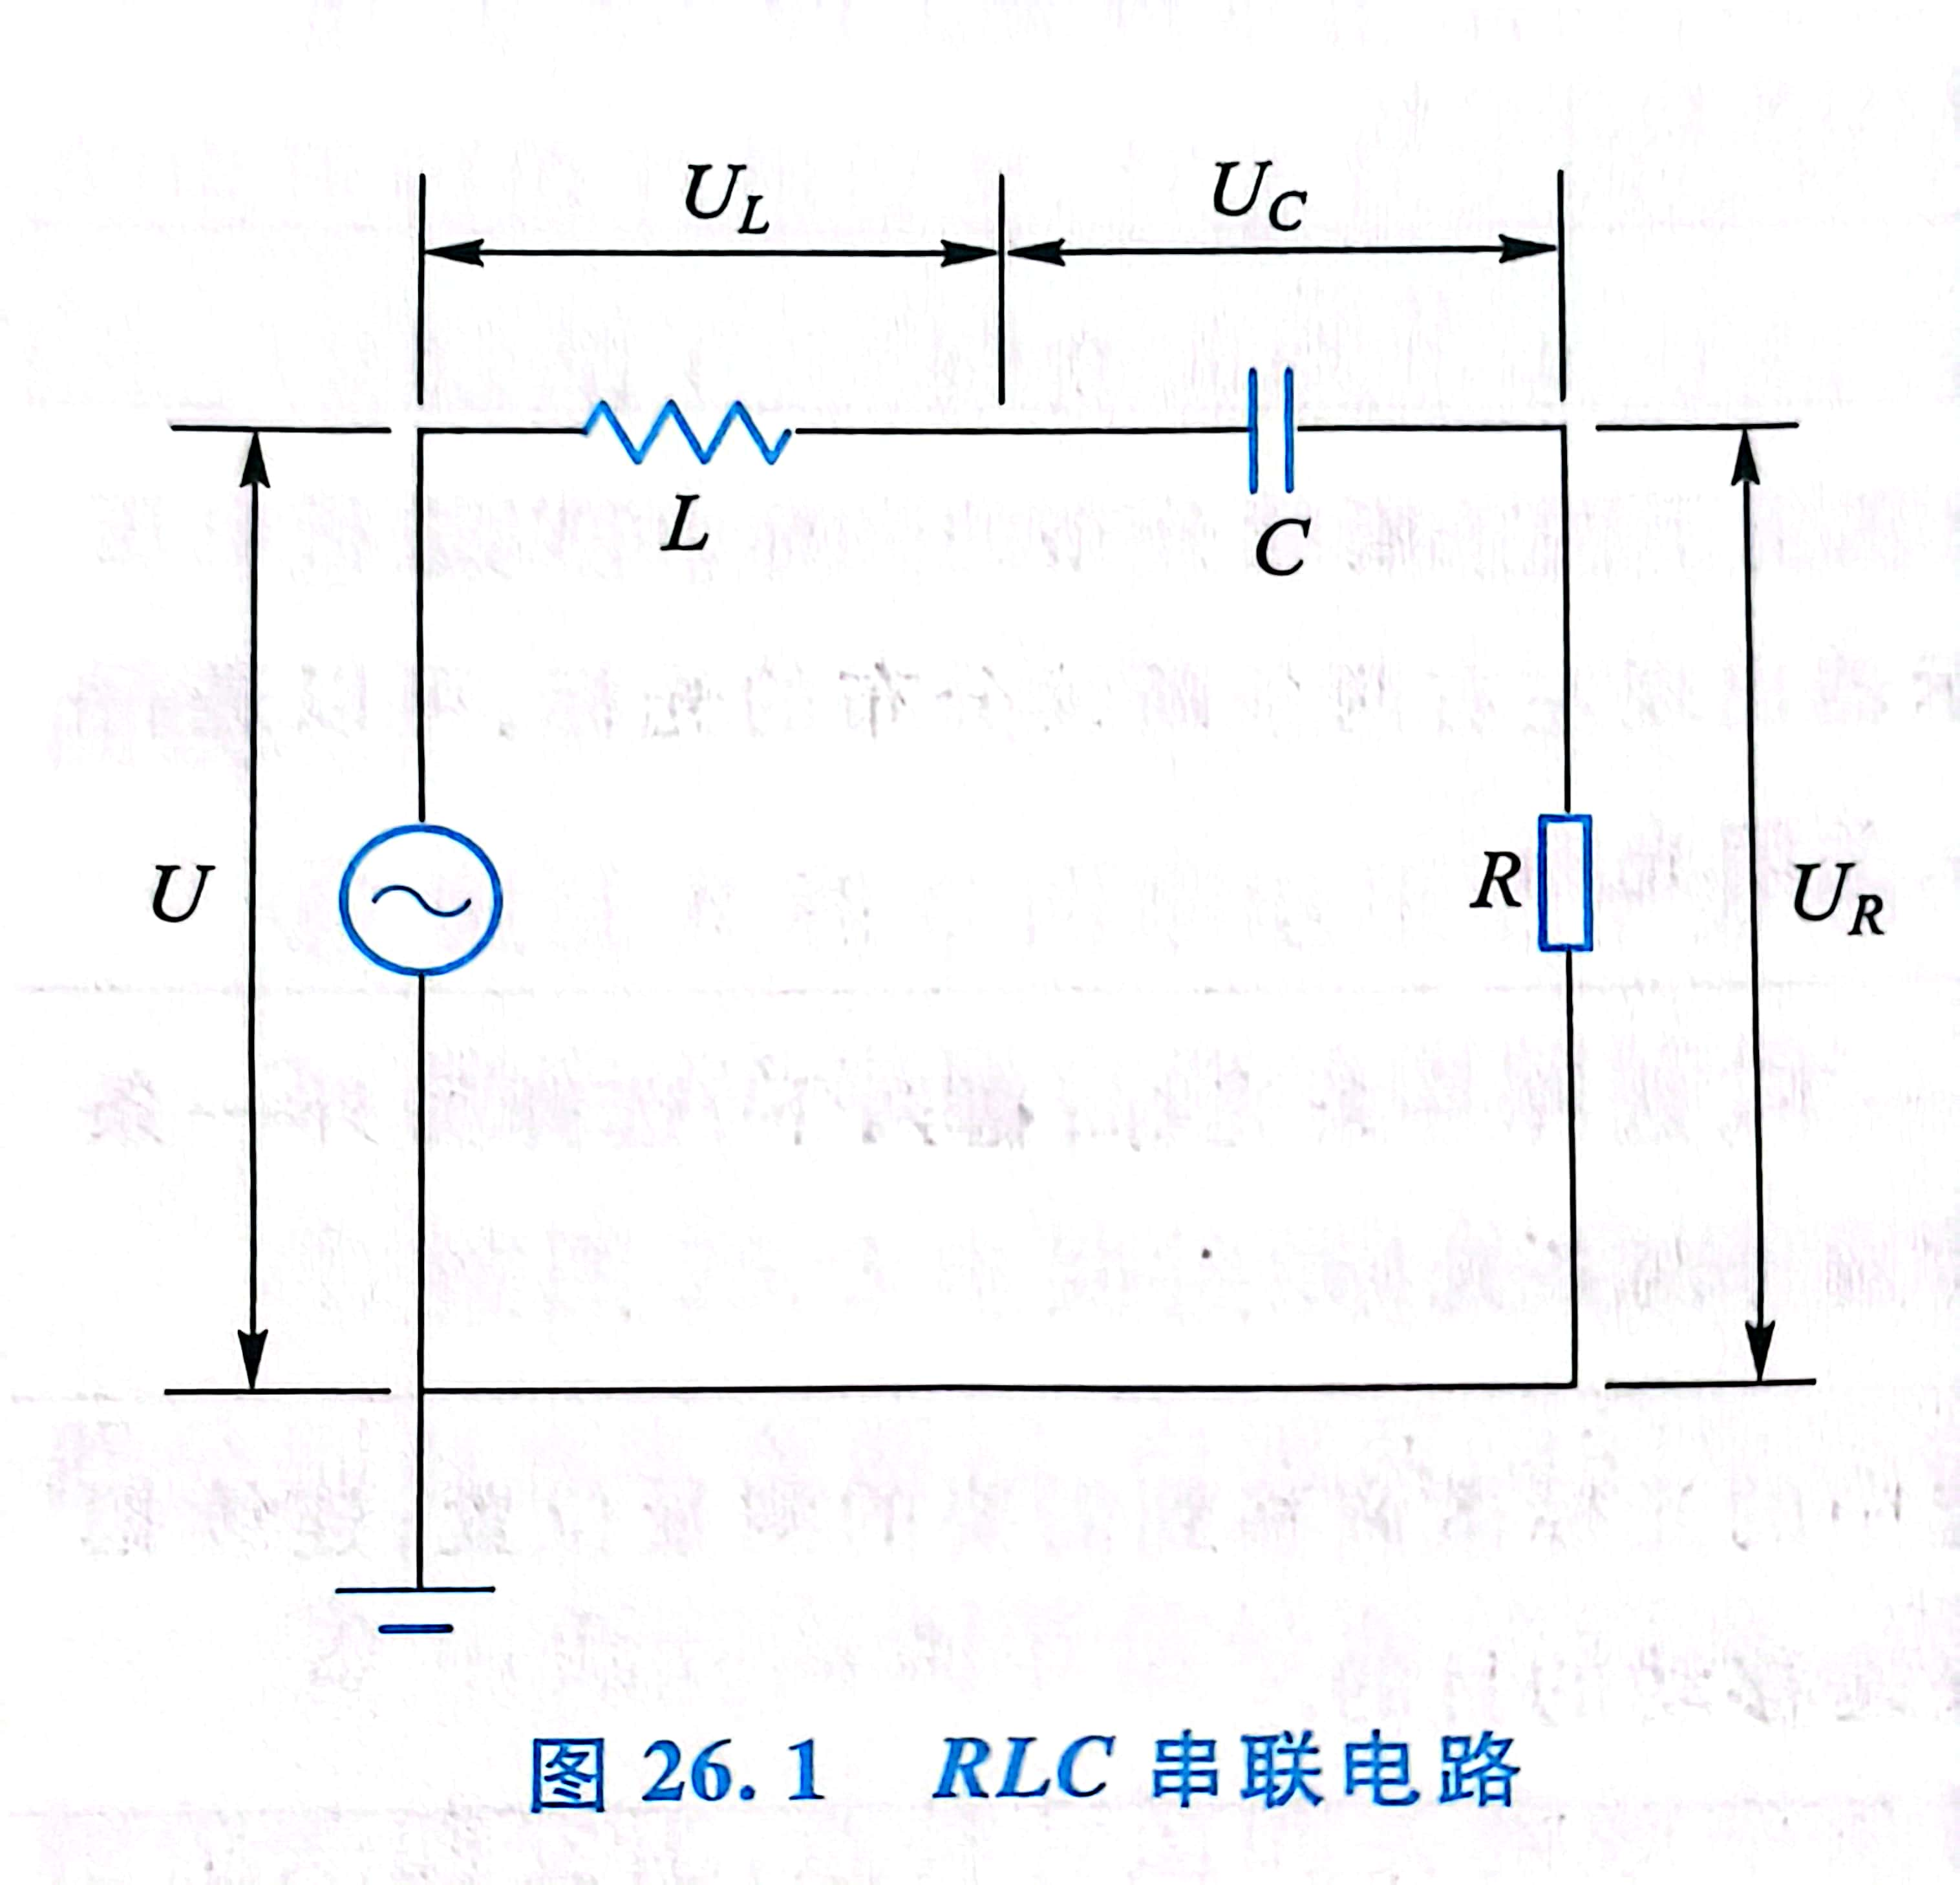
\includegraphics[width=\textwidth]{RLCdianlu.jpg}
  \end{minipage}
  \hfill
  \begin{minipage}[H]{0.4\textwidth}\label{rlcwentaitexing}
  \centering
  \caption{RLC稳态特性}
  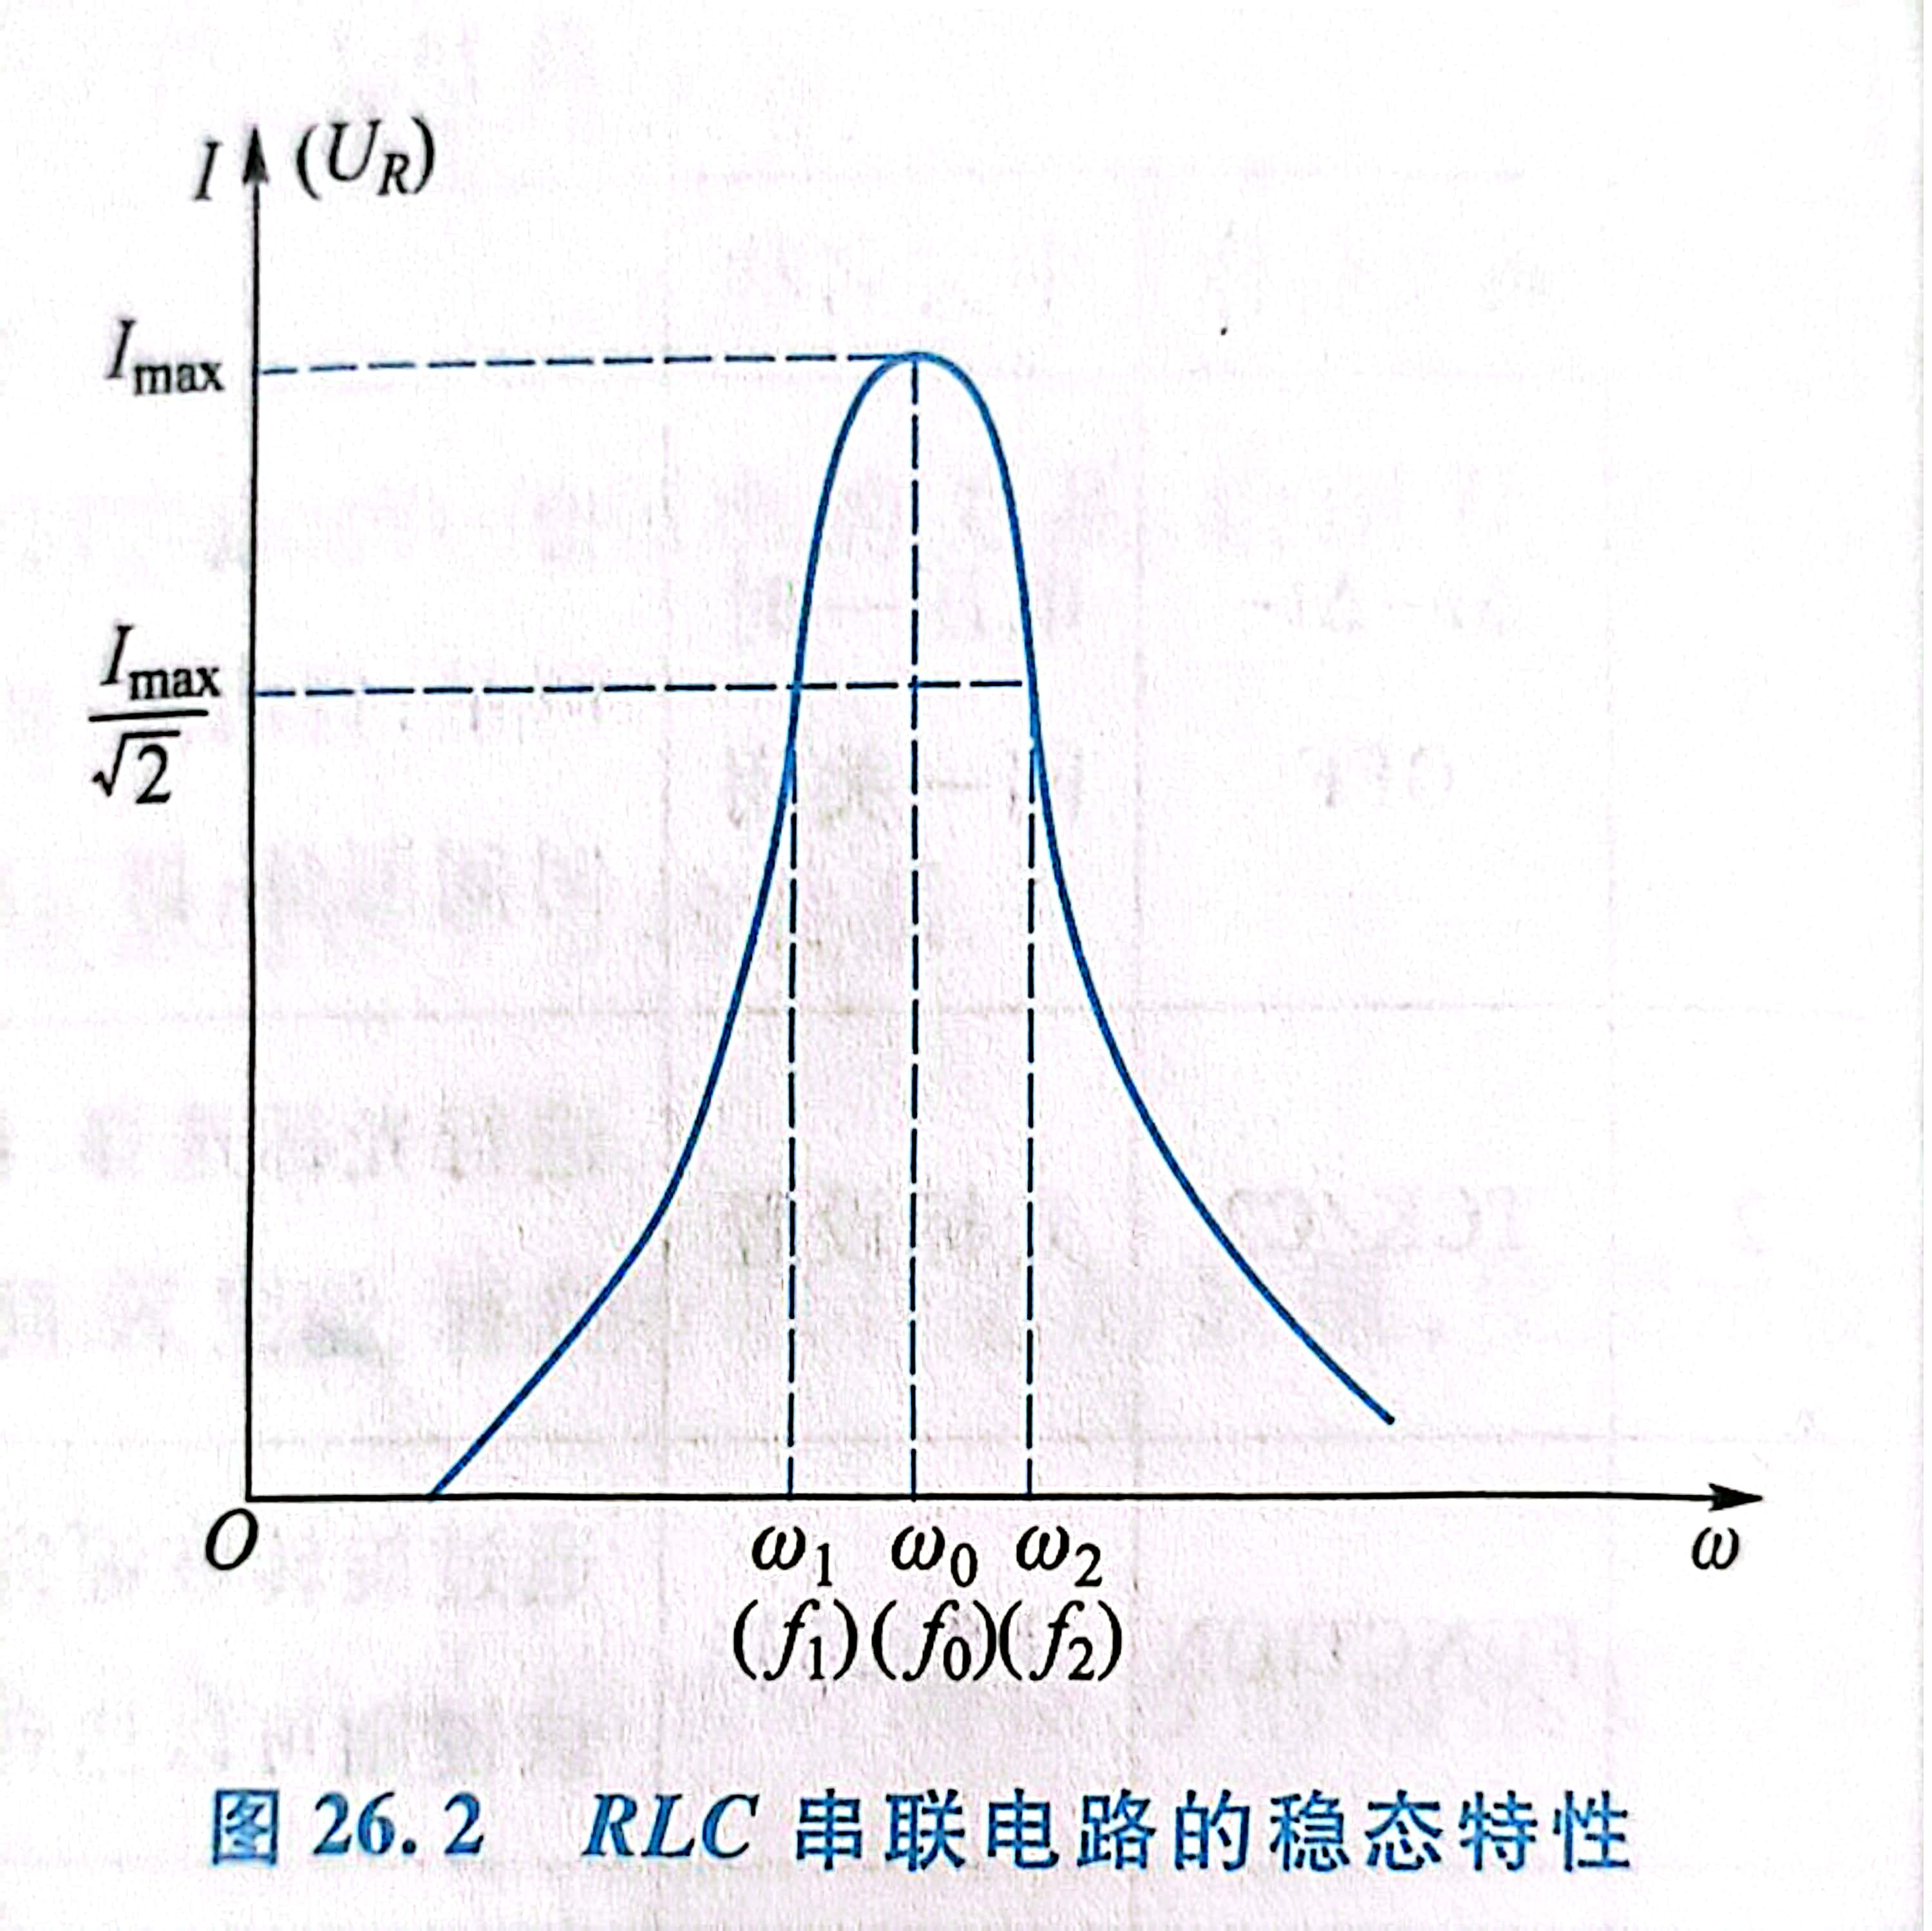
\includegraphics[width=\textwidth]{RLCwentaitexing.jpg}
  \end{minipage}
\end{figure}

\section{实验原理}
  \subsection{RLC传来内电路的幅频特性和相频特性}
  如图\ref{rlcdianlu},进行电路的连接。在电路中,电感线圈和电容器两者本身也具有损耗,
  和电阻在电路中的效果一样。
  所以现在设电感线圈和电容器两者串联后具有等效损耗电阻为$R_{L}$,则依照假设及电路,
  RLC电路中的总阻抗为
  \begin{equation}\label{rlczongzukang}
    Z=\sqrt{(R+R_{L})^2+(\omega L-\frac{1}{\omega C})^2}
  \end{equation}
  同时也能得出回路中的电流大小为
  \begin{equation}\label{rlcdianliu}
    I=\frac{U}{\sqrt{(R+R_{L})^2+(\omega L-\frac{1}{\omega C})^2}}
  \end{equation}

  保持总电压U不变,则会得到图\ref{rlcwentaitexing}所示的RLC串联电路的幅频特性曲线。
  由于欧姆定律$U=IR$,所以$U_{R}-\omega \mbox{和} I-\omega$关系是相同。因此实验
  中经常测量的是$U_{R}-\omega$曲线。

  实验中总电压和电流之间的相位差设为$\varphi$,可以表达为
  \begin{equation}\label{phibiaodashi}
    \varphi = \arctan \frac{\omega L-\frac{1}{\omega C}}{R+R_{L}} 
  \end{equation}
  
  \begin{wrapfigure}[13]{l}{4.5cm}\label{rlcxiangpintexing}
    \centering
    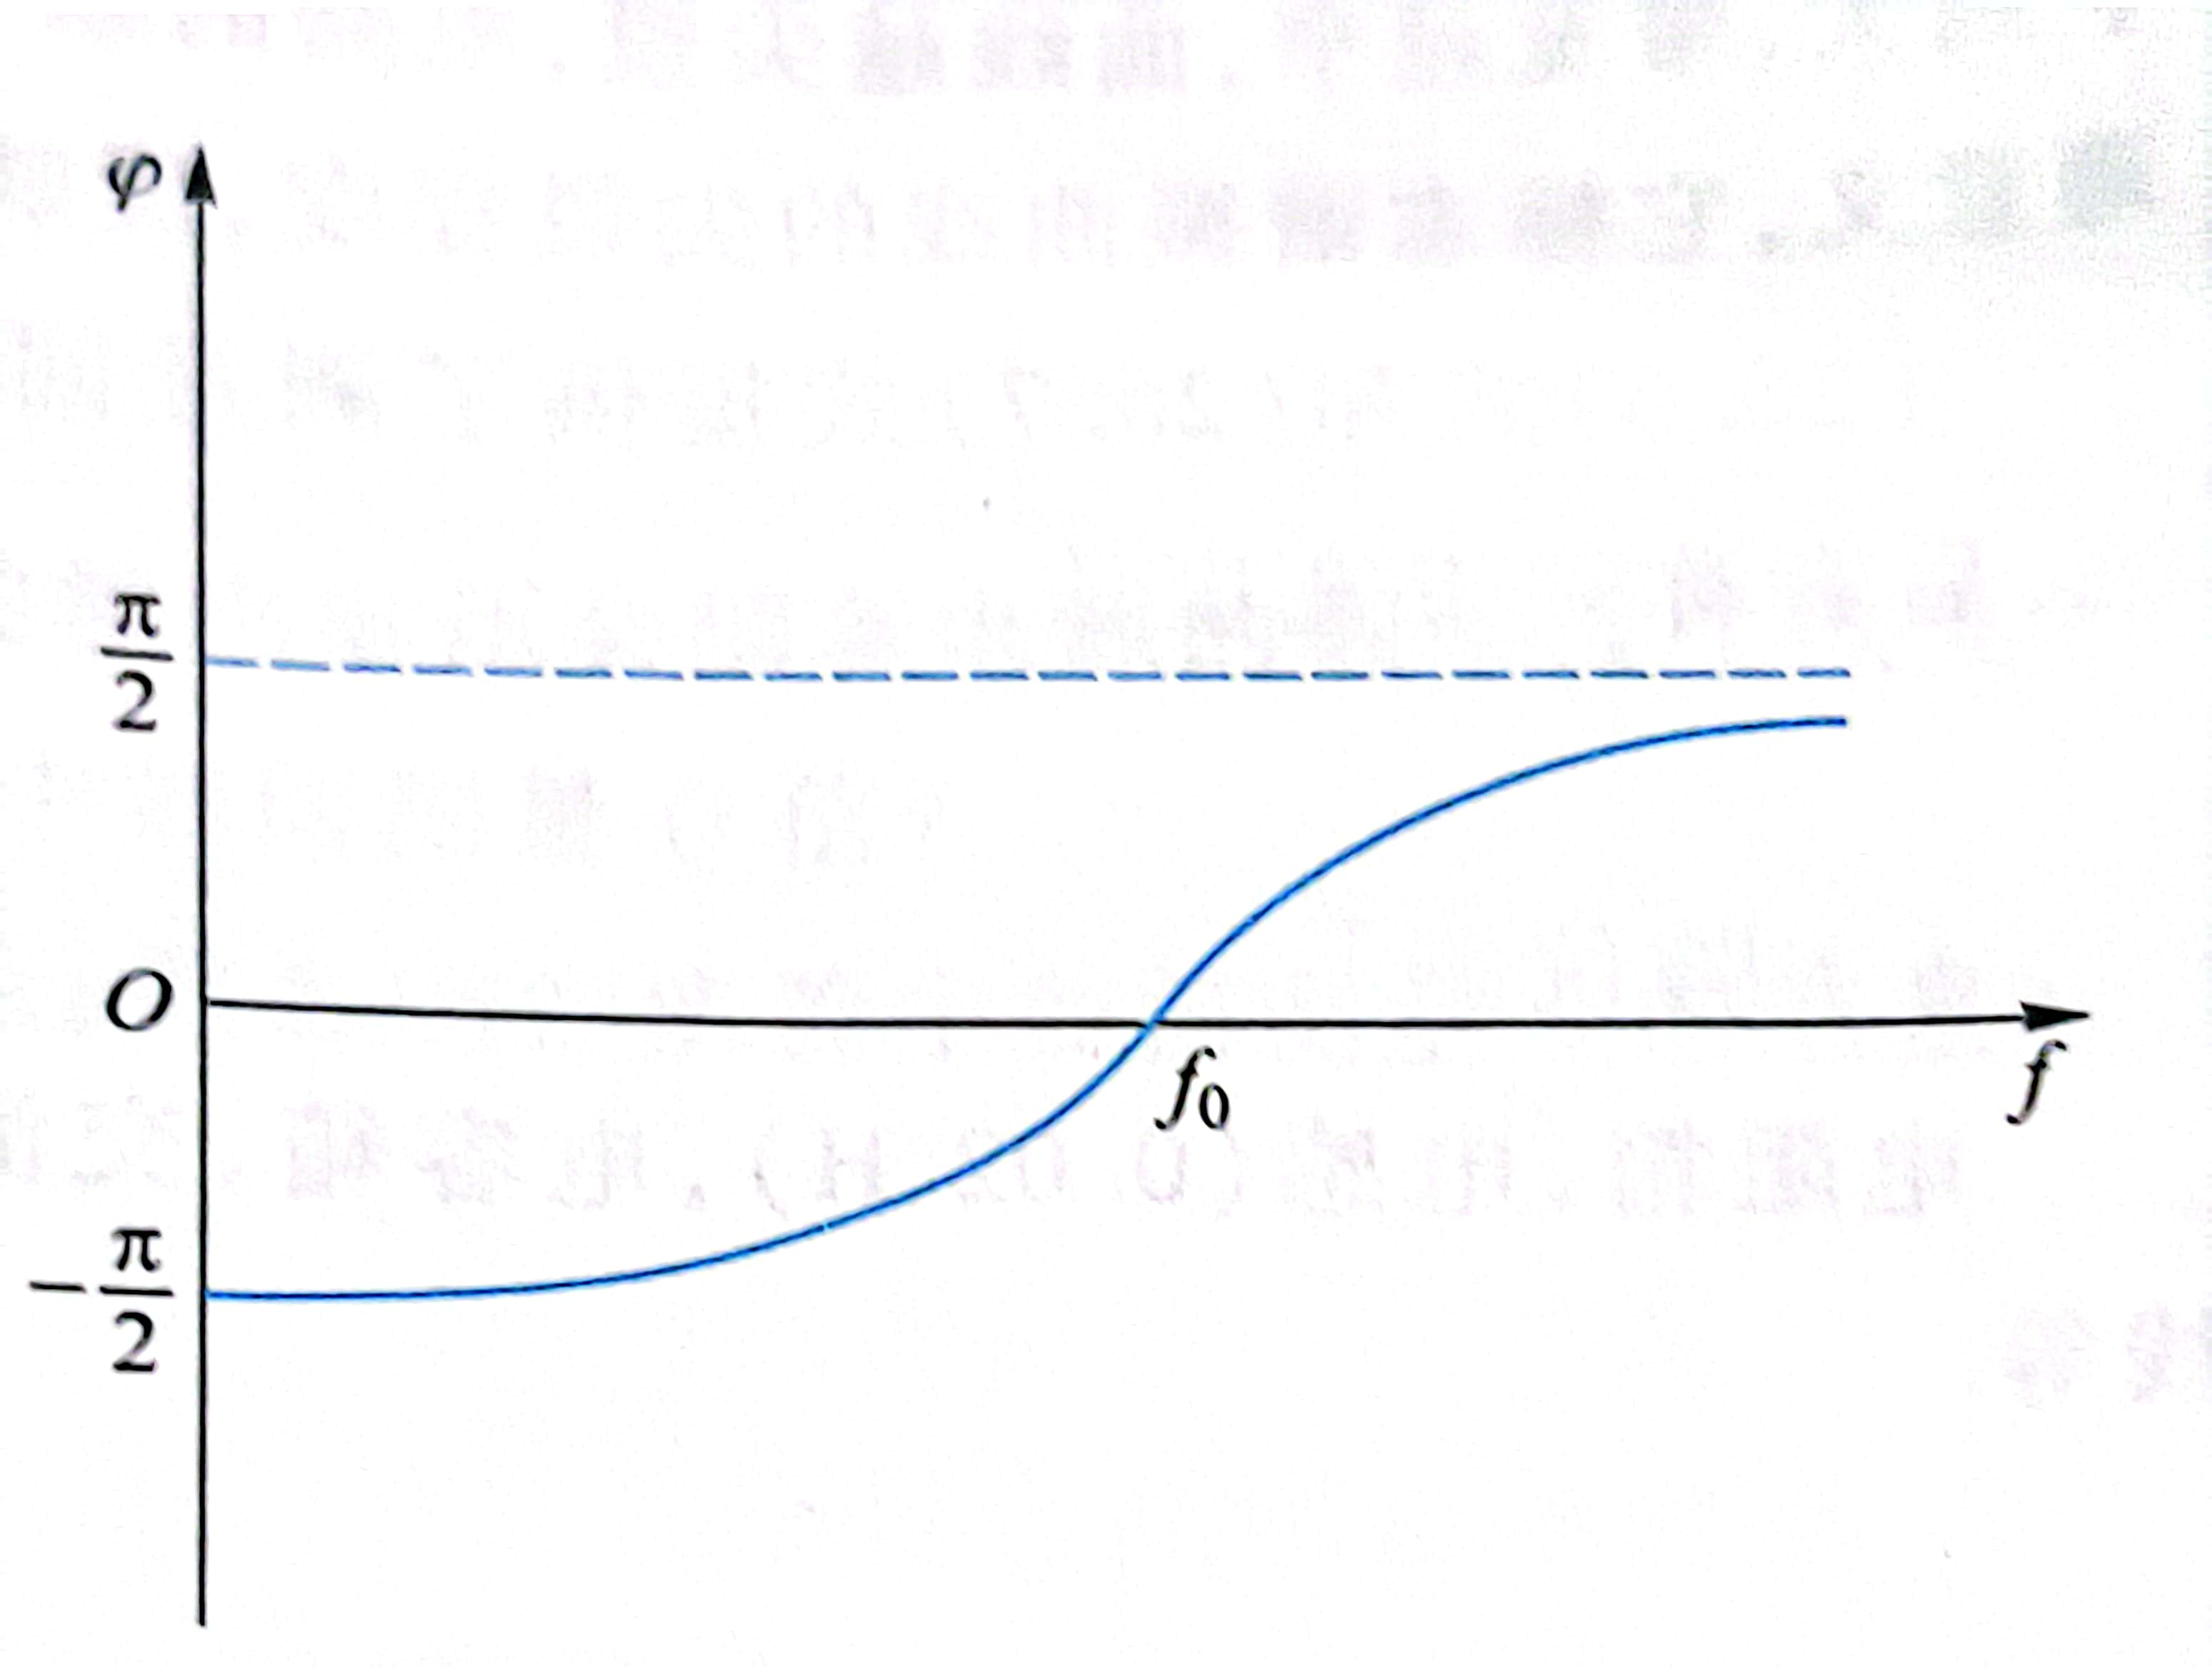
\includegraphics[width=0.3\textwidth,height=0.3\textheight]{RLCxiangpintexing.jpg}
    \caption{RLC相频特性}
  \end{wrapfigure}
  而实验中理论上应该出现的相位差随着电源频率变化关系如图\ref{rlcxiangpintexing}所展示的那样。
  从图\ref{rlcxiangpintexing}中以及$\varphi$的表达式式\ref{phibiaodashi}可以得出以下结论:

  1.\quad  当$\omega L > \frac{1}{\omega C}$时,有$\varphi > 0$,电流的相位落后于电源电压,整个电路
            呈现电感性,随着频率的增加$\varphi$越来越接近$\frac{\pi}{2}$。
            电感性的意思就是:
            电感性是指导体中的电流变化时会引起该导体中的自感应电动势的性质。
            从物理意义上看,电感性是描述导体中电磁场的建立和消散过程。当电流在导体中变化时,
            围绕导体的磁场也随之变化,而磁场的变化又会在导体内部感应出电动势,这个过程就体现了电感性。

  2.\quad  当$\omega L < \frac{1}{\omega C}$时,有$\varphi < 0$,电流的相位超前于电源电压,整个电路
            呈现电容性,随着频率的减小,$\varphi$越来越接近$\frac{\pi}{2}$。
            电容性是指导体对电荷的储存能力的一种性质。
            从物理意义上讲,电容性反映了导体中的电荷和电势之间的关系。当在导体上的两点之间存在电势差时,
            会在导体的两点附近聚集对应量的正负电荷,这种聚集电荷的能力就是电容性。

  3.\quad  当$\omega L = \frac{1}{\omega C}$时,有$\varphi < 0$,电流相位等于电源电压。整个电路
            处于谐振状态,此时回路中电流达到最大,记作$I_{max}$,令$\omega_{0}\mbox{和}f_{0}$分别表示
            $\varphi = 0$时候的角频率和频率,并分别成为谐振角频率和谐振频率,也可以表达为
            \begin{equation}
              \omega_{0}=\frac{1}{\sqrt{LC}} \mbox{,} f_{0}=\frac{1}{2\pi \sqrt{LC}}
            \end{equation}
  
  \subsection{RLC串联谐振电路的品质因素Q}
  当RLC串联谐振的时候,也就是出现当$\omega L = \frac{1}{\omega C}$时,
  有$\varphi < 0$,电流相位等于电源电压的时候,$U_{L}=U_{C}$,即纯电感和理想电容两端的电压相等,而
  \begin{equation}
    U_{L}=I_{max}\omega_{0}L=\frac{U}{R+R_{L}}\omega_{0} L=\frac{U}{R+R_{L}}\sqrt{\frac{L}{C}}
  \end{equation}
  令$Q=\frac{1}{R+R_{L}} \sqrt{\frac{L}{C}}$则有
  \begin{equation}\label{qyiyi}
    U_{L}=U_{C}=QU
  \end{equation}
  Q称为串联谐振电路的品质因数,式中的U为信号源的输出电压,如果Q>>1,则$U_{L}$和$U_{C}$都远大于信号源电压。
  这种现象叫做RLC电路的电压谐振。Q值反映了谐振电路的特性,由式\ref{qyiyi}得到Q的一个物理意义:
  电压谐振时,电路呈纯电阻性,纯电感和理想电容两端的电压均为信号源电压的Q倍。

  为了描述$I-\omega$谐振曲线的尖锐程度,通常规定I由最大值$I_{max}$下降到$\frac{I_{max}}{\sqrt{2}}$时
  对应的频率$\omega_{1}$和$\omega_{2}(\omega_{1}<\omega_{0}<\omega_{2})$之差称为“通频带宽都”,与$\omega_{0}$
  和回路的品质因数Q之间的关系为
  \begin{equation}\label{qyiyi2}
    Q=\frac{\omega_{0}}{\omega_{2} - \omega_{1}}=\frac{f_{0}}{f_{2}-f_{1}}
  \end{equation}
  Q越大,带宽越窄,曲线越尖锐,电路的频率选择性越好,由此得到的Q值的第二个物理意义:它标志谐振曲线的尖锐
  程度,反映电路对频率的选择性。

  式\ref{qyiyi}和式\ref{qyiyi2}提供了测量回路Q值的原理和方法,前者称为电压谐振法,后者称为频带宽度法。

\section{实验装置器材介绍}
电阻箱、电感(0.02H)、电容箱、交流信号源、交流毫伏表、双通道示波器、导线等

\section{实验内容及实验步骤}
  \subsection{测量RLC串联电路的幅频特性和相频特性}
  \ding{172} 按照图\ref{rlcdianlu}连接电路,选择合适LC的数值。

  \ding{173} 使用示波器的两个通道同时观察电源和电阻两端的电压,根据公式先估算以下电路的谐振频率$F_{0}$,
              然后调节信号源的频率,观察电阻两端电压岁频率的变化规律,确定测量频率范围。

  \ding{174} 以一定的频率间隔从低到高改变频率,每一个频率测量点测量电阻两端的电压$U_{R}$和电阻两端
              电压与电源电压之间的相位差$\varphi_{R}$,在测量过程中注意保持电源电压幅值的稳定。

  \ding{175} 绘制RLC串联电路的谐振曲线$U_{R}-f\mbox{和}\varphi_{R}-f$

  \subsection{测量回路的品质因数Q值}
  \ding{172} 当电路处于谐振状态时,将电容与电阻交换位置,测量电容两端的电压$U_{C}$。或将电感和电阻交换位置,
              测量电感两端的电压$U_{L}$,计算品质因数Q。

  \ding{173} 在$U_{R}-f$图上画出RLC串联电路的频带宽度,并计算Q值。

  \ding{174} 将Q的测量值和计算值进行比较。
\newpage

\section{实验原始数据}
% \begin{figure}[H]
%   \centering
%   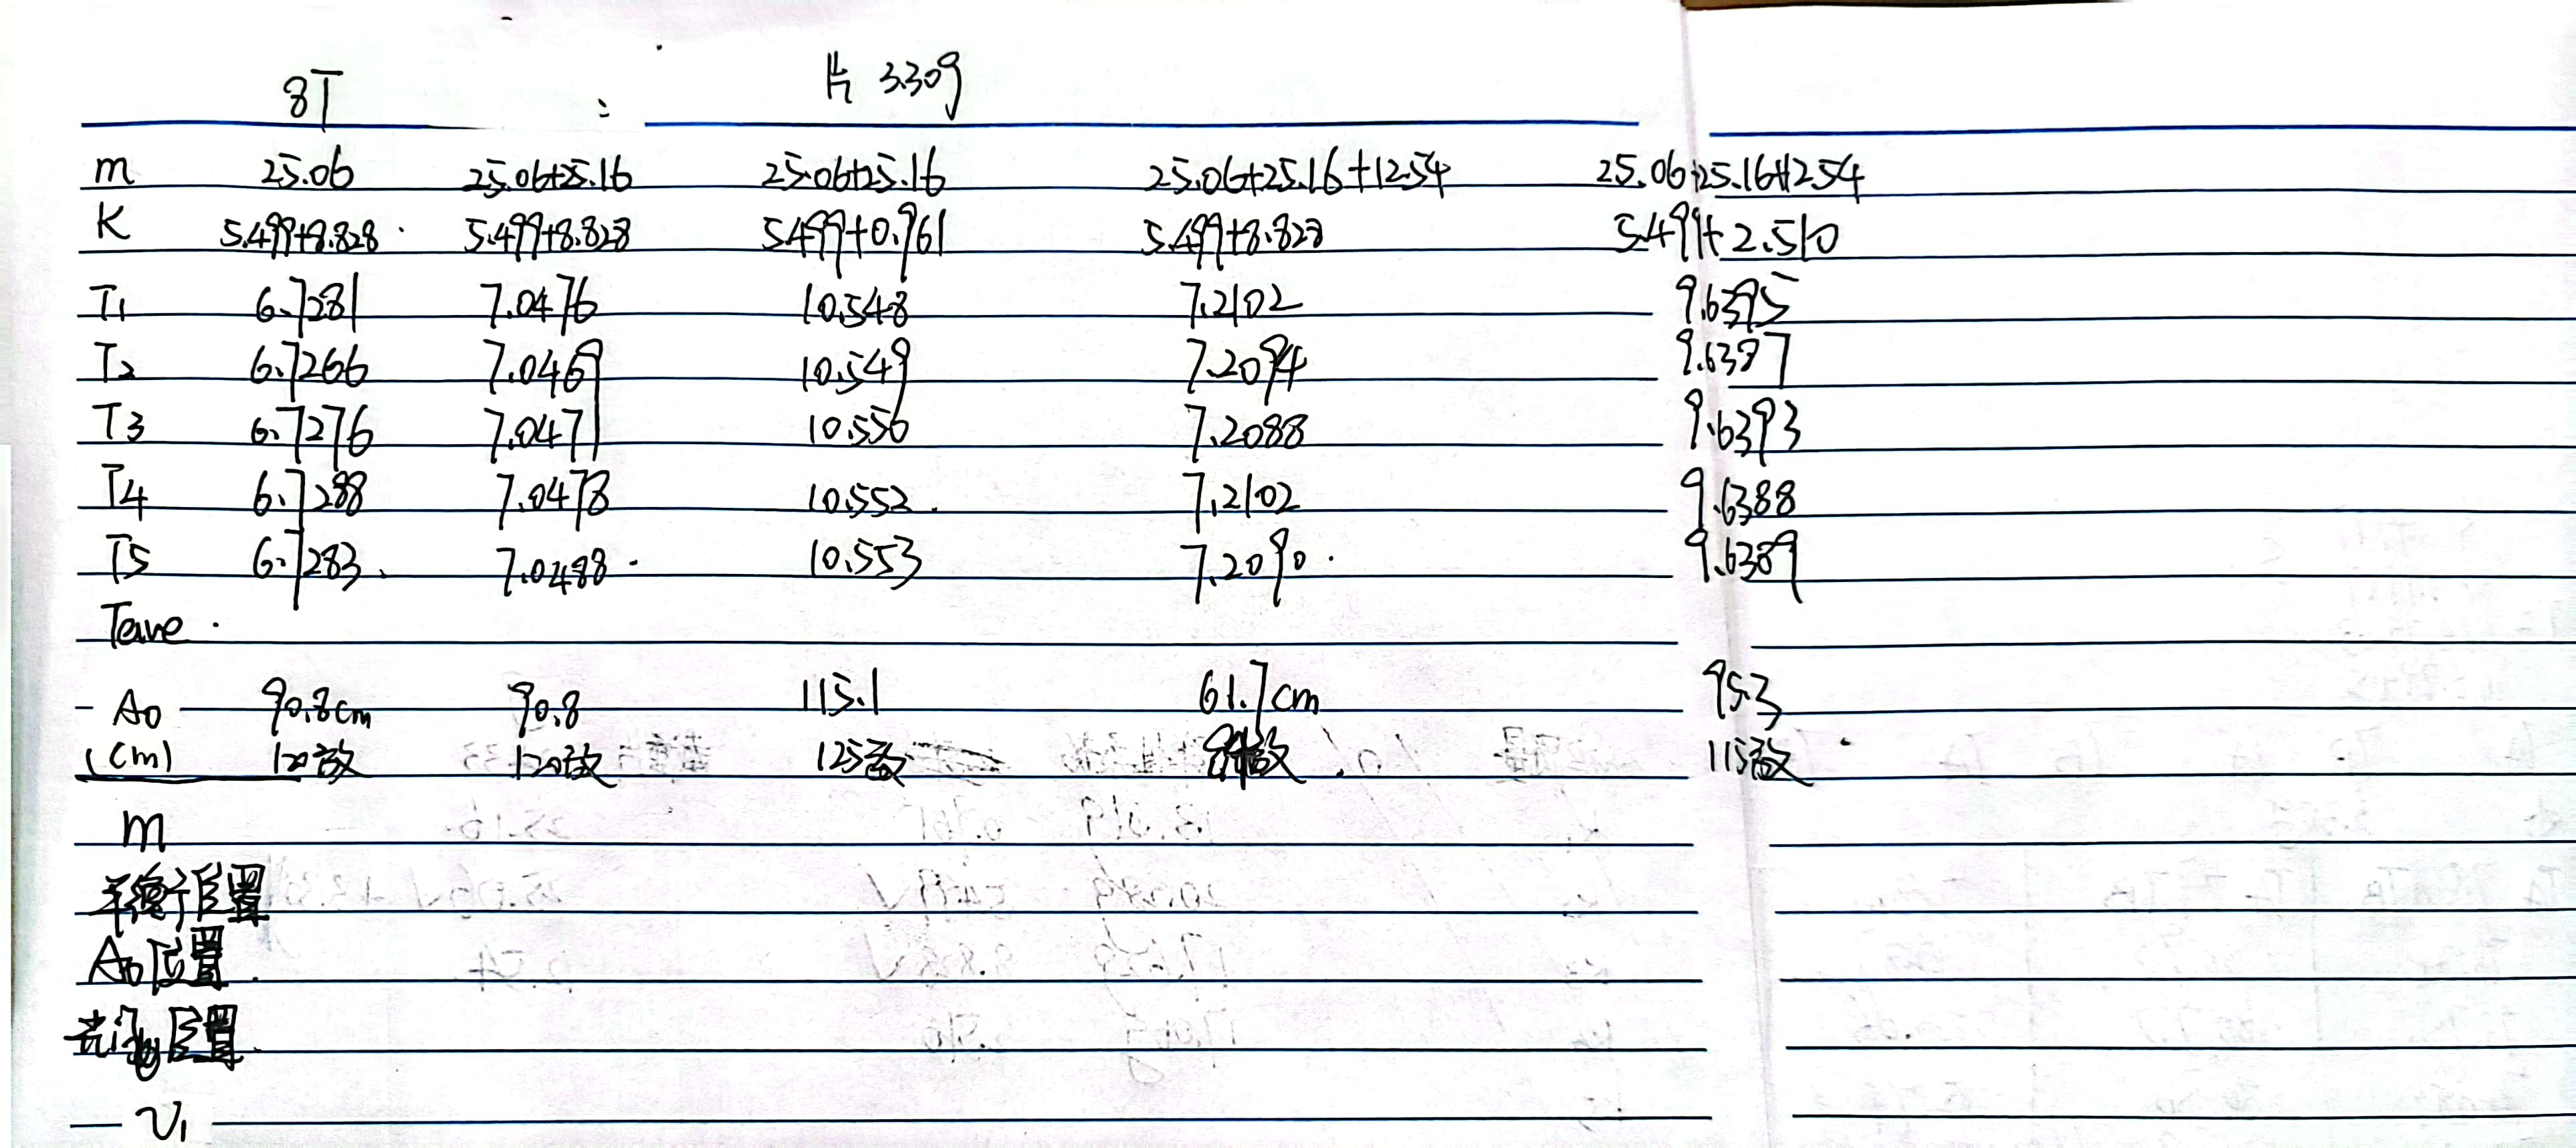
\includegraphics[width=0.9\textwidth,height=0.8\textheight]{yuanshishujv1.jpg}
%   \caption{实验原始数据1}
% \end{figure}
% \newpage
% \begin{figure}[H]
%   \centering
%   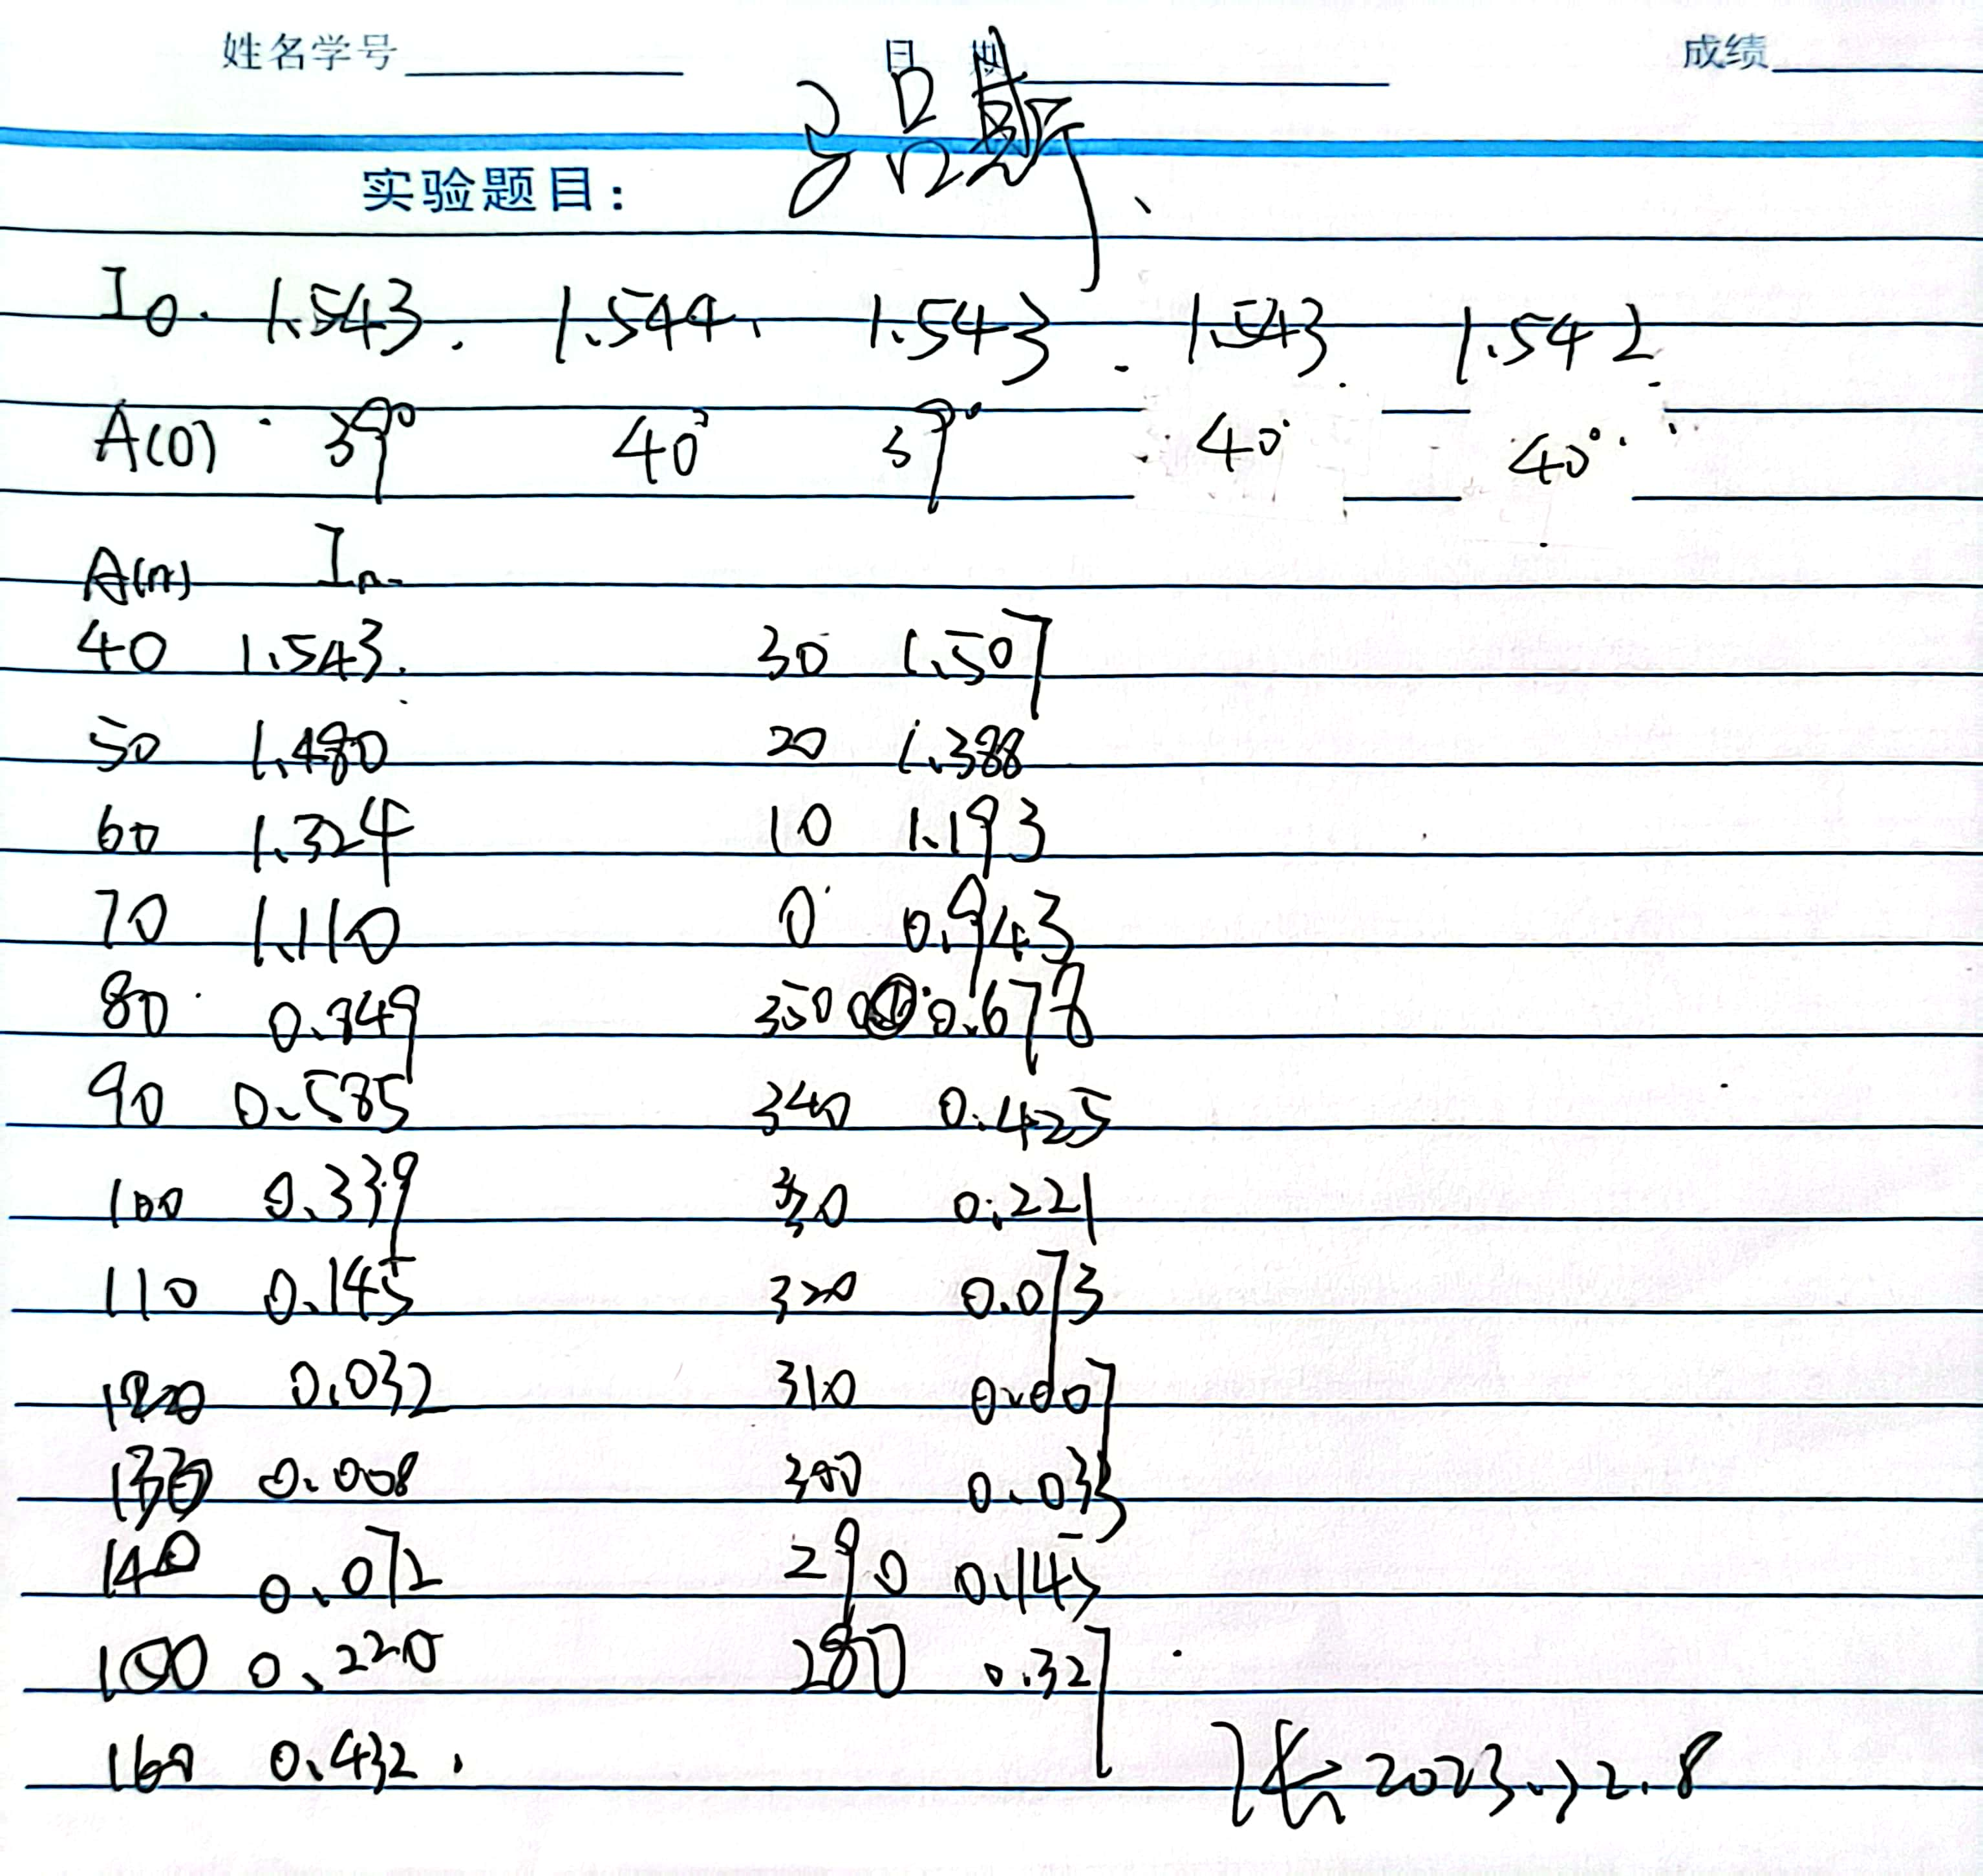
\includegraphics[width=0.9\textwidth,height=0.8\textheight]{yuanshishujv2.jpg}
%   \caption{实验原始数据2}
% \end{figure}
% \newpage
% \begin{figure}[H]
%   \centering
%   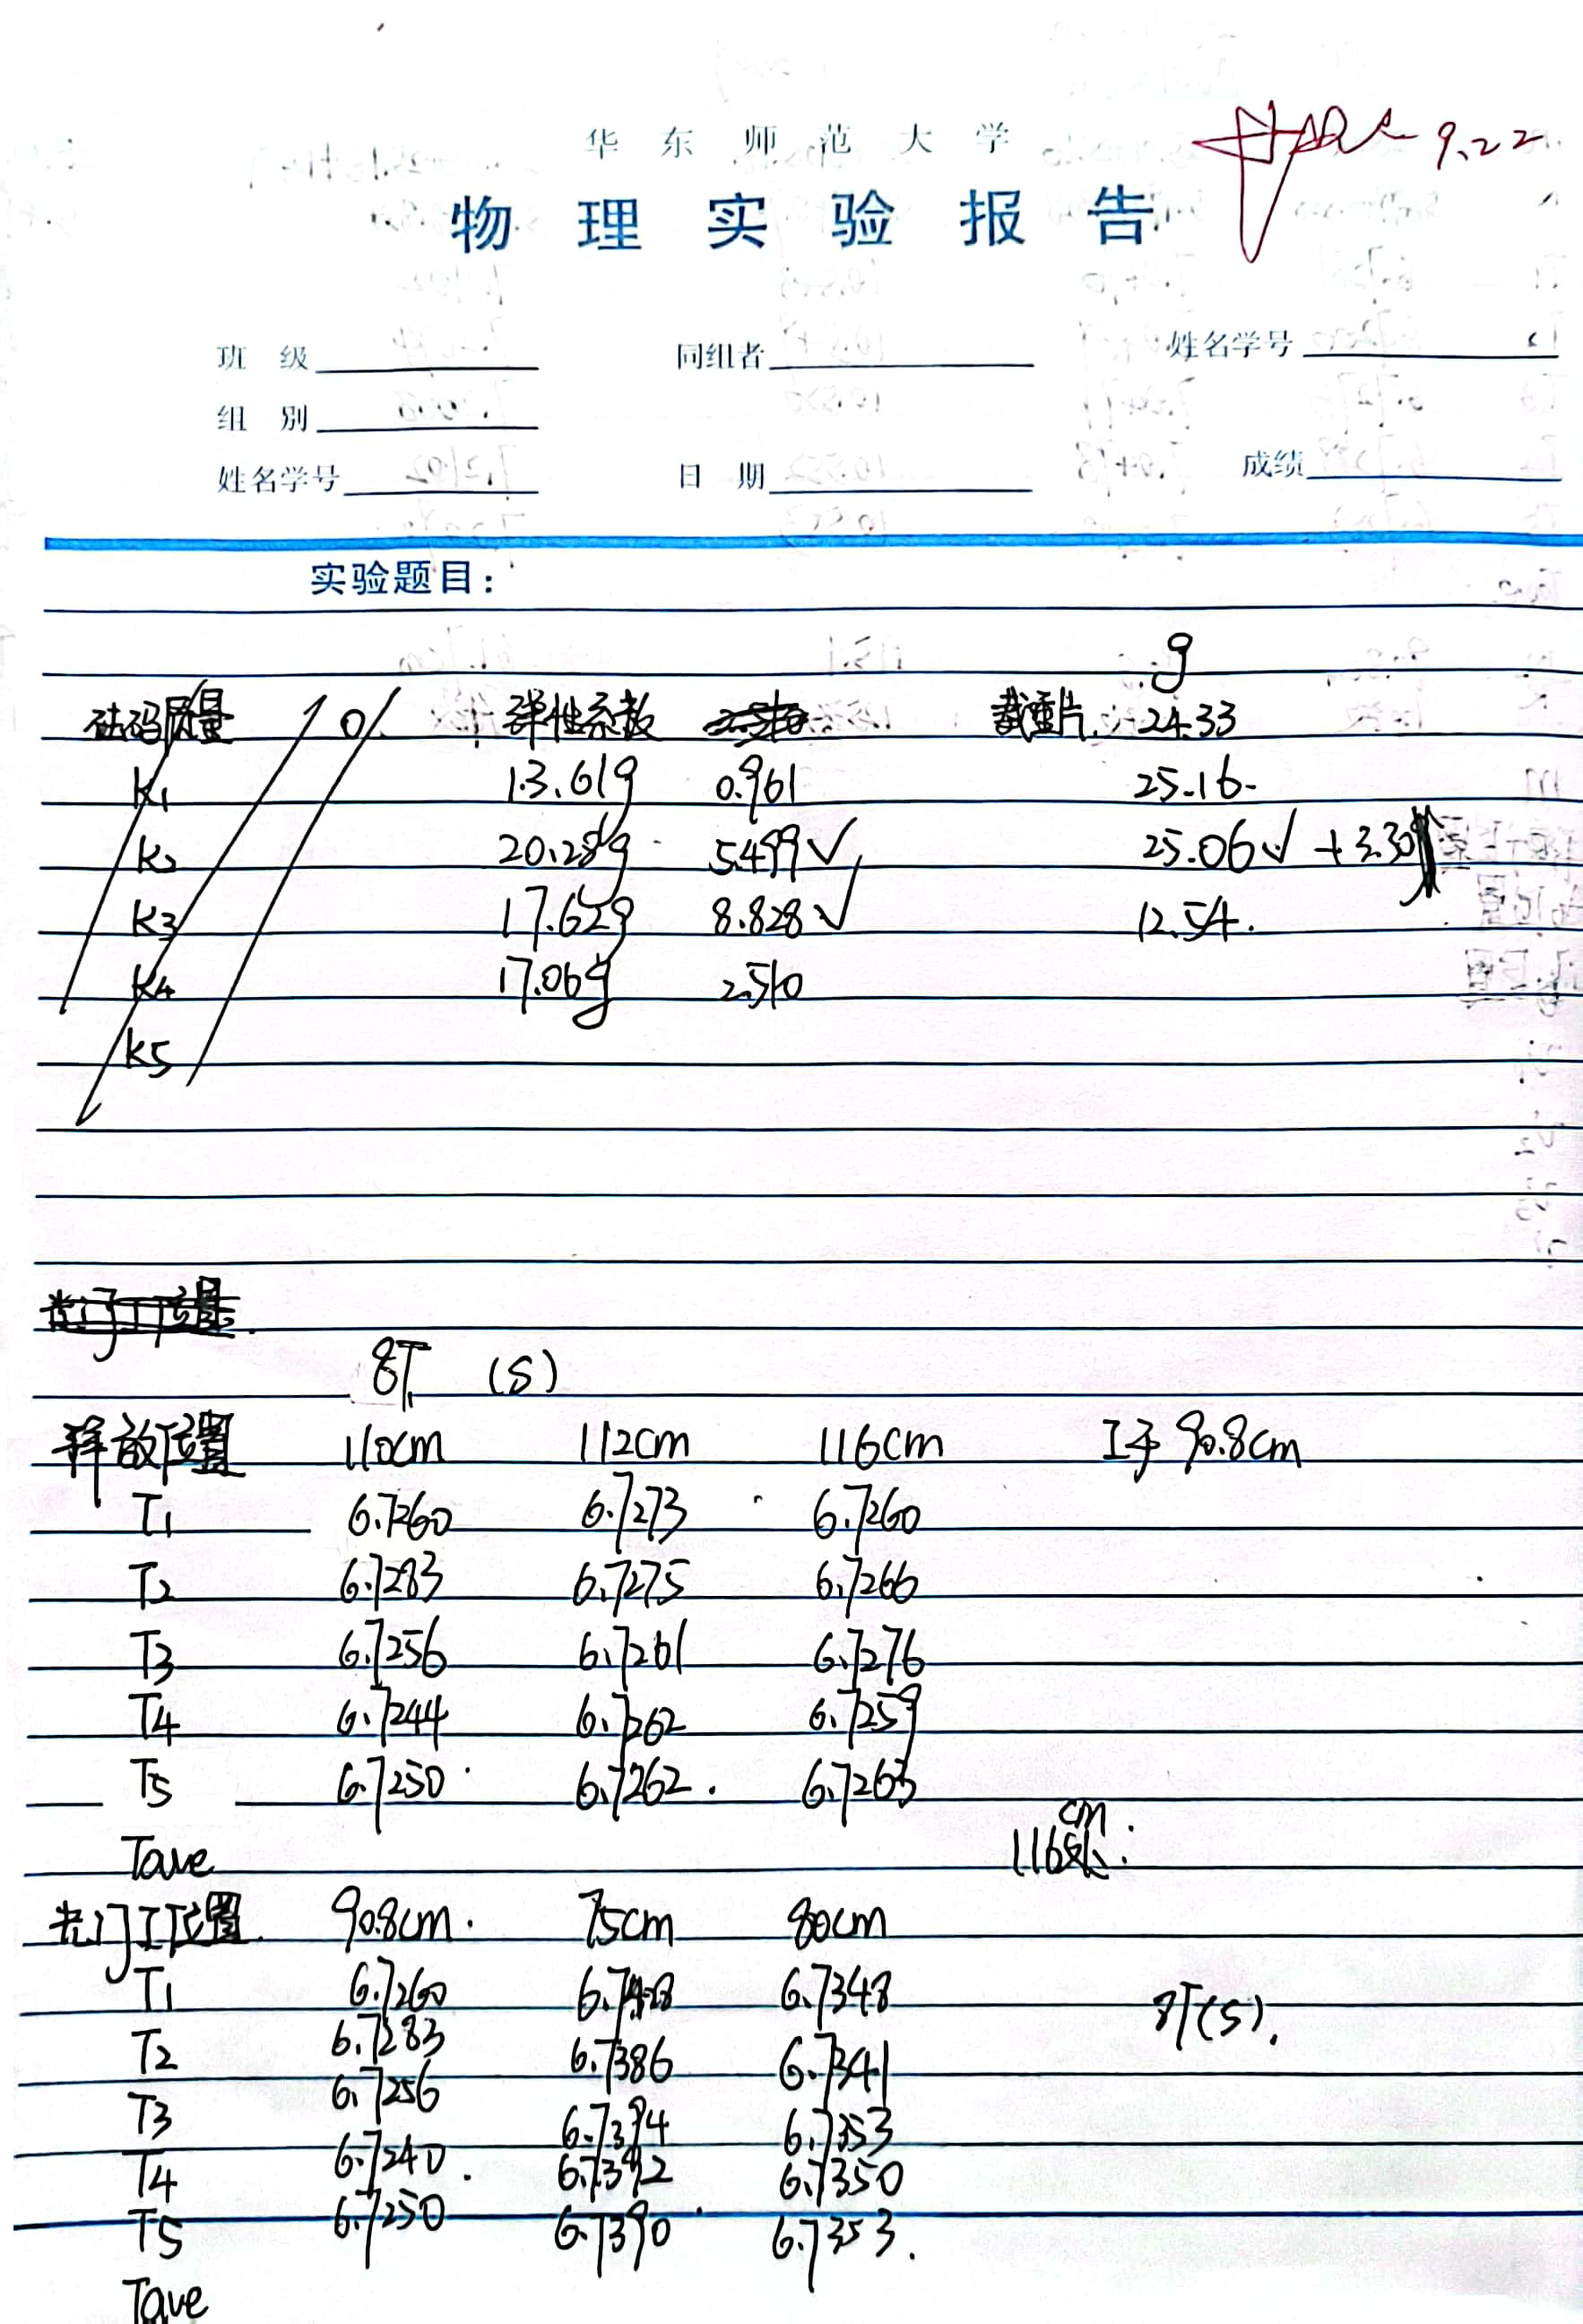
\includegraphics[width=0.9\textwidth,height=0.8\textheight]{yuanshishujv3.jpg}
%   \caption{实验原始数据3}
% \end{figure}
\newpage

\section{实验数据处理}
  \subsection{测量RLC串联电路的幅频特性和相频特性}
%   \begin{wrapfigure}[4]{l}{4cm}\label{dianzushujv}
%     \centering
%     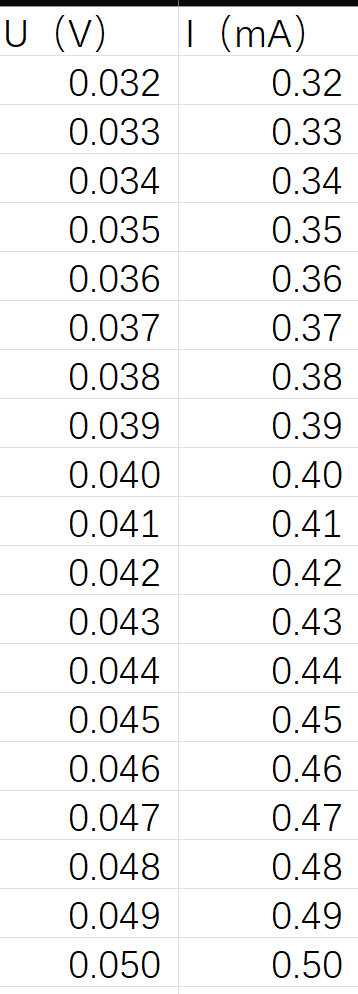
\includegraphics[width=0.1\textwidth,height=0.4\textheight]{dianzushujv.png}
%     \caption{电阻数据}
%   \end{wrapfigure}

%   实验中测得的电阻导通数据如图\ref{dianzushujv}。对数据进行处理最终得到图\ref{dianzuzuotu}。

%   \begin{figure}[H]\label{dianzuzuotu}
%     \centering
%     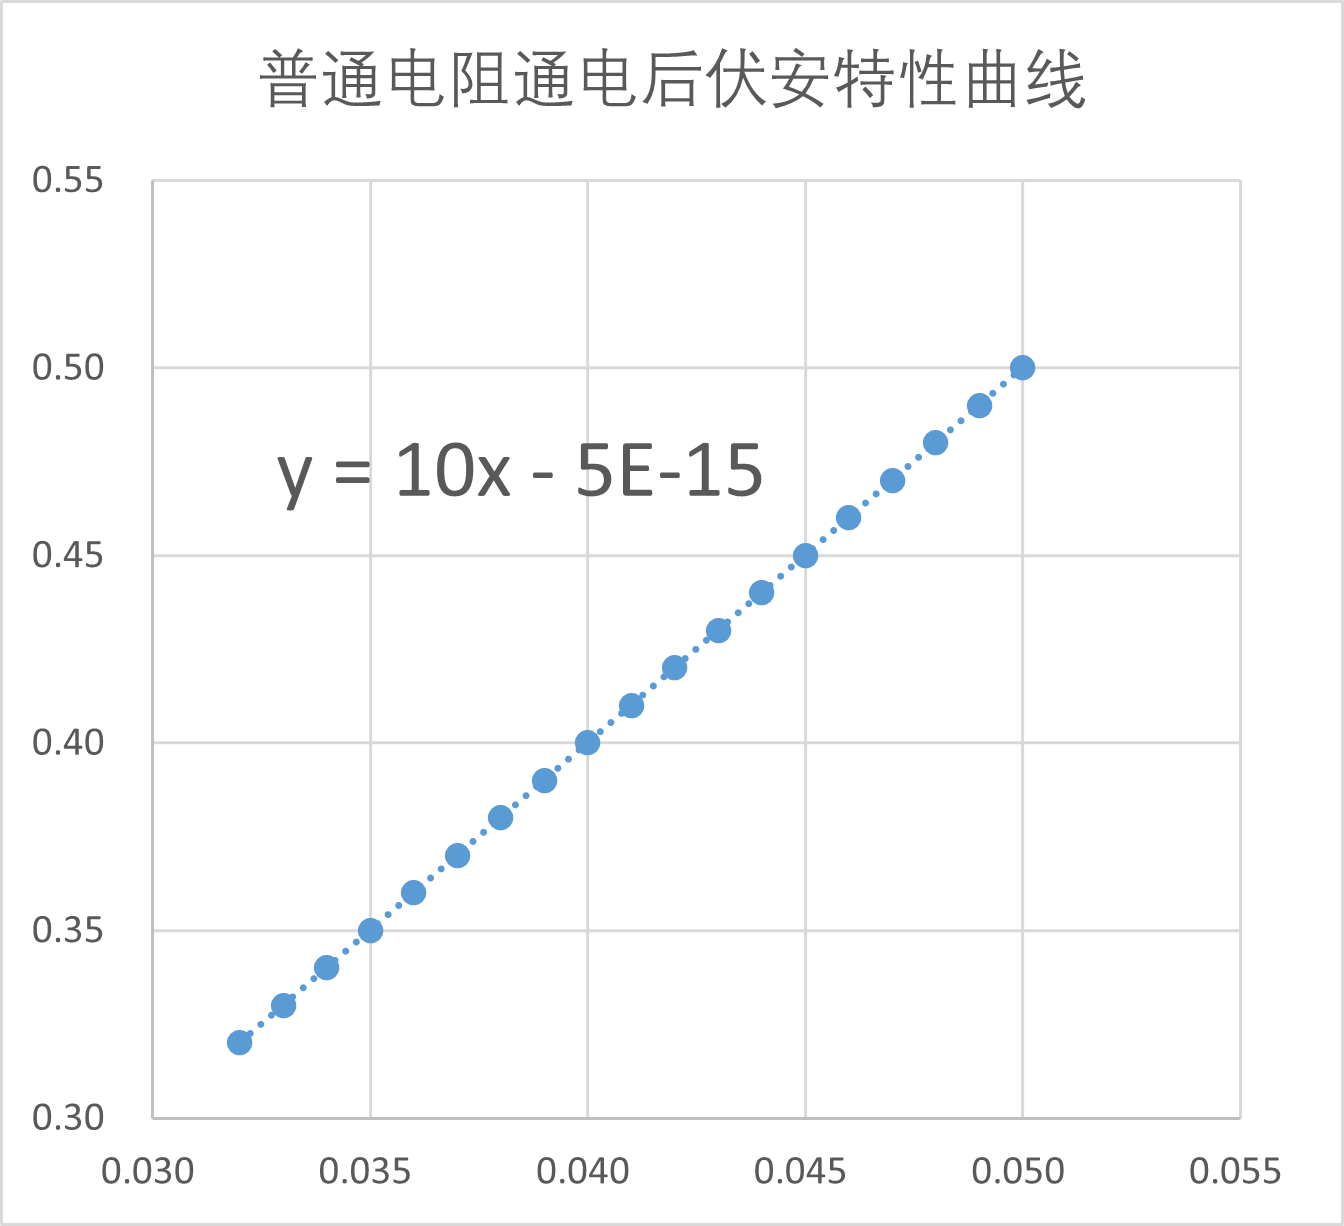
\includegraphics[width=0.4\textwidth,height=0.3\textheight]{dianzuzuotu.png}
%     \caption{电阻结果作图}
%   \end{figure}

%   最终得到的实验结果较为满意,基本符合欧姆定律,可能由于测量时间较短,所以电阻发热不严重没有
%   影响其阻值,得到的伏安特性曲线也是较为完美的直线。实验较为成功。

%   \subsection{测量普通二极管的正向伏安特性曲线}
%   \begin{wrapfigure}[2]{l}{4cm}\label{putongshujv}
%     \centering
%     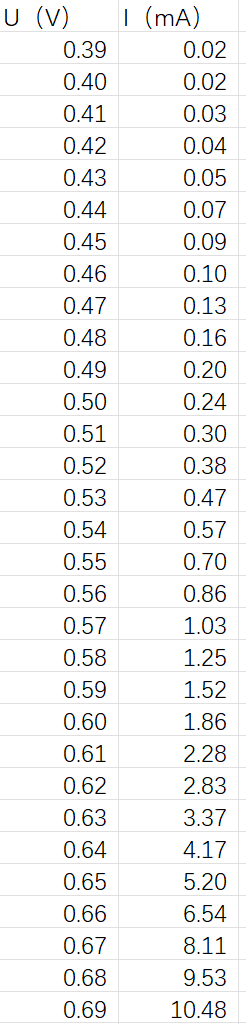
\includegraphics[width=0.1\textwidth,height=0.3\textheight]{putongshujv.png}
%     \caption{普通二极管数据}
%   \end{wrapfigure}

%   实验中测得的普通二极管
%   伏安特性曲线数据如图\ref{putongshujv}。对数据进行处理最终得到图\ref{putongzuotu}。

%   \begin{figure}[H]\label{putongzuotu}
%     \centering
%     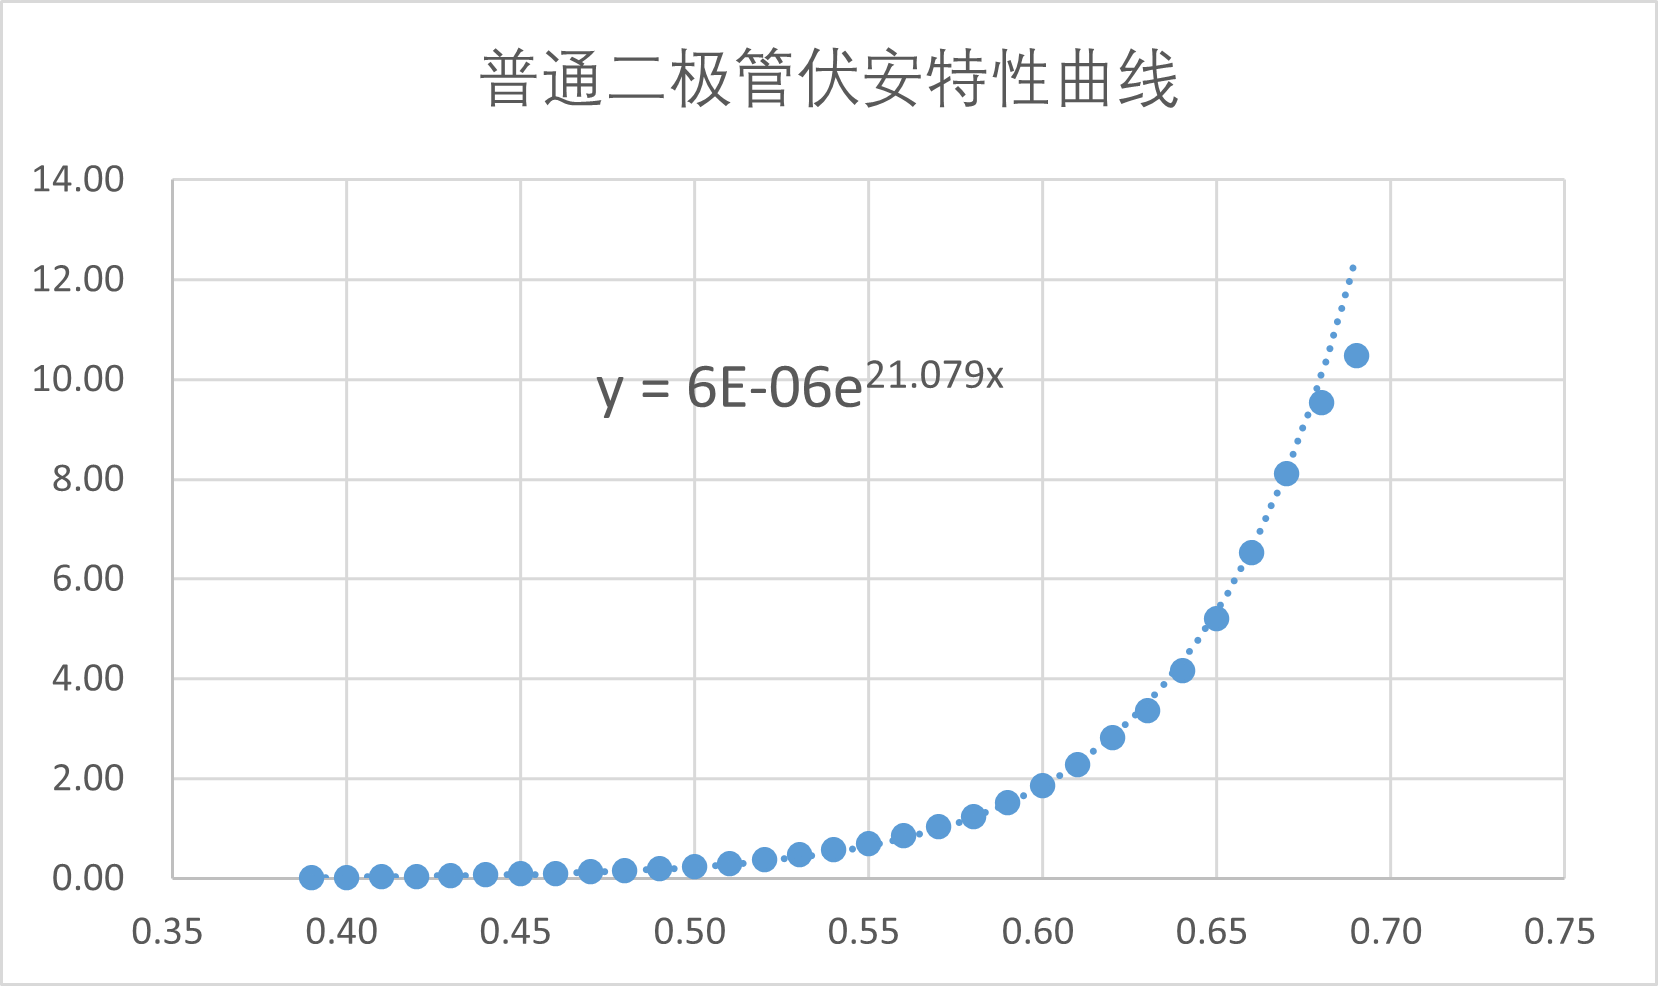
\includegraphics[width=0.4\textwidth,height=0.3\textheight]{putongzuotu.png}
%     \caption{普通二极管伏安特性曲线作图}
%   \end{figure}

%   最终得到的实验结果表明整个实验数据得到的图形基本符合非线性元件的e为底的指数曲线拟合结果。
%   \subsection{测量稳压二极管伏安特性曲线}
%   实验包括两部分,一部分是正向导通的情况下的伏安特性曲线,另一部分是反向导通的情况下的伏安特性曲线。
  
%   \subsubsection{测量稳压二极管的正向伏安特性曲线}

%   \begin{wrapfigure}[4]{l}{4cm}\label{wenyazhengxiangshujv}
%     \centering
%     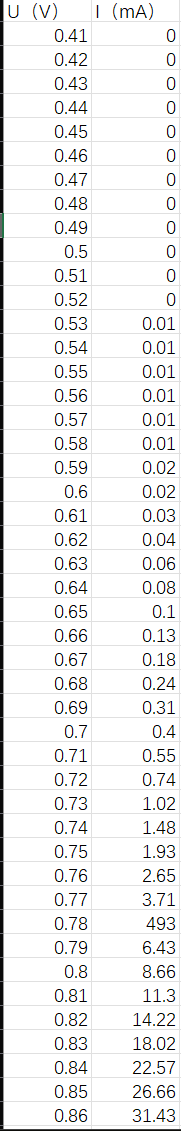
\includegraphics[width=0.1\textwidth,height=0.4\textheight]{wenyazhengxiangshujv.png}
%     \caption{稳压二极管正向导通数据}
%   \end{wrapfigure}
%   实验中测得的稳压二极管正向导通的时候的
%   伏安特性曲线数据如图\ref{wenyazhengxiangshujv}。对数据进行处理最终得到图\ref{wenyazhengxiangzuotu}。
%   \begin{figure}[H]\label{wenyazhengxiangzuotu}
%     \centering
%     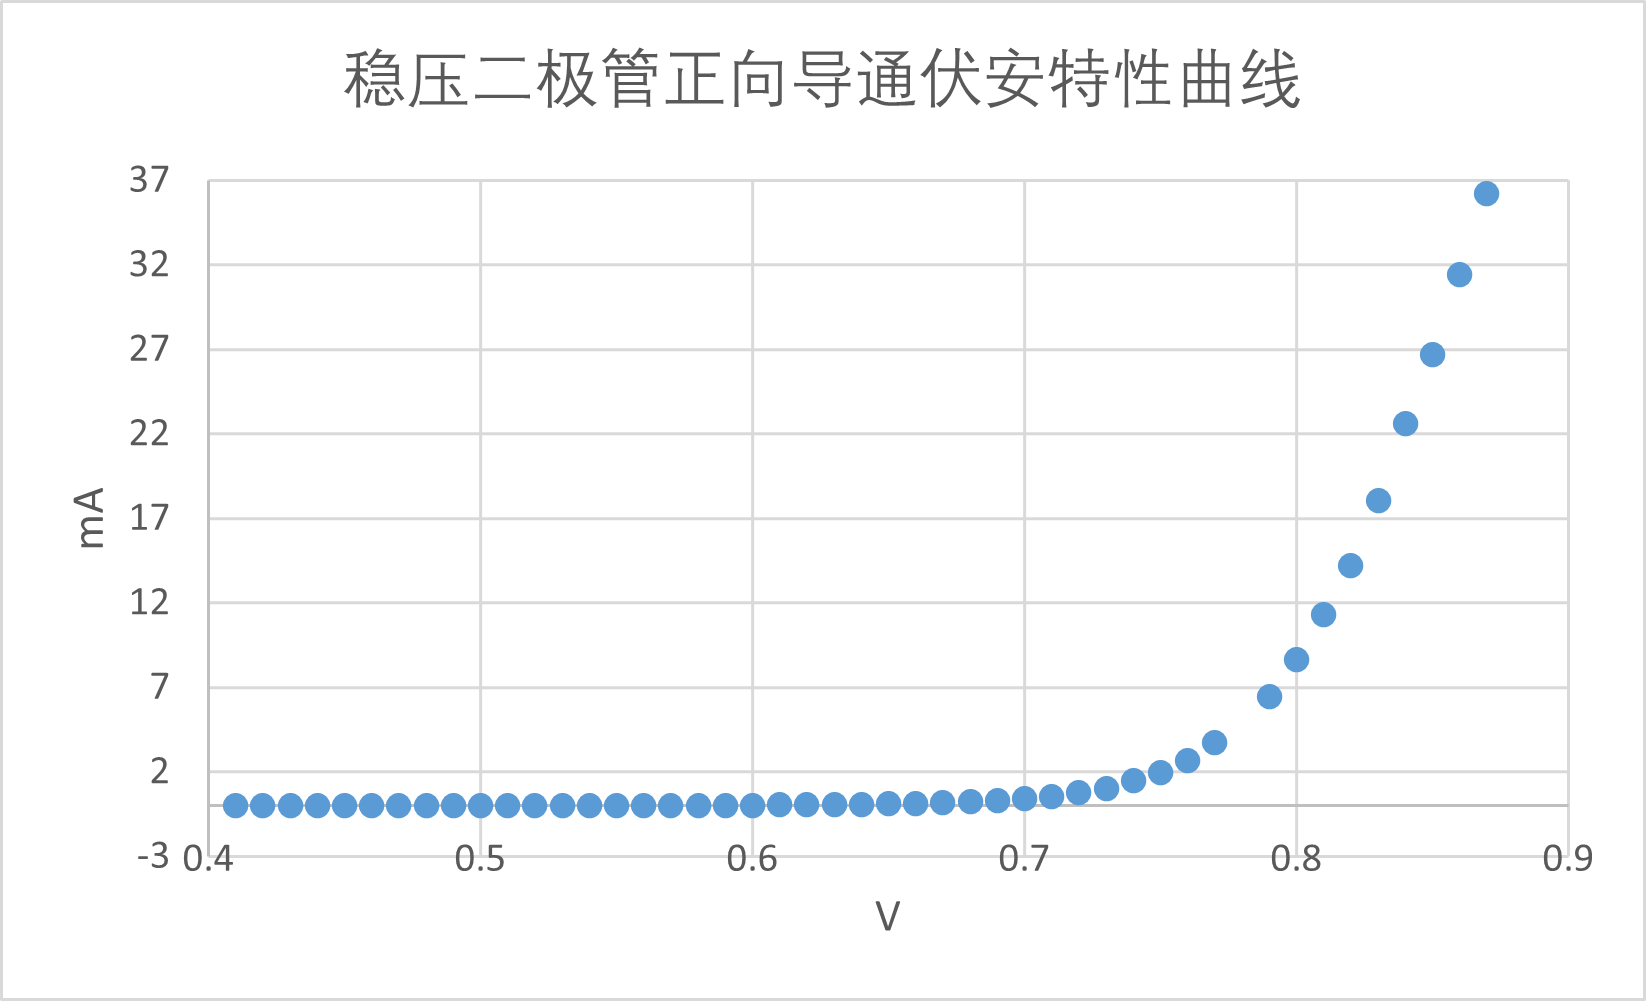
\includegraphics[width=0.4\textwidth,height=0.3\textheight]{wenyazhengxiangzuotu.png}
%     \caption{稳压二极管正向导通伏安特性曲线作图}
%   \end{figure}

%   \subsubsection{测量稳压二极管的反向伏安特性曲线}

%   \begin{wrapfigure}[3]{l}{4cm}\label{wenyafanxiangshujv}
%     \centering
%     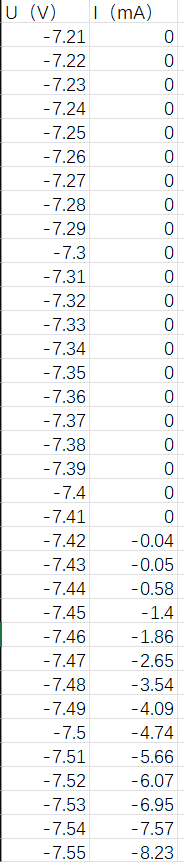
\includegraphics[width=0.3\textwidth,height=0.4\textheight]{wenyafanxiangshujv.png}
%     \caption{稳压二极管反向导通数据}
%   \end{wrapfigure}
%   实验中测得的稳压二极管反向导通的时候的
%   伏安特性曲线数据如图\ref{wenyafanxiangshujv}。对数据进行处理最终得到图\ref{wenyafanxiangzuotu}。
%   \newpage
%   \begin{figure}[h]\label{wenyafanxiangzuotu}
%     \centering
%     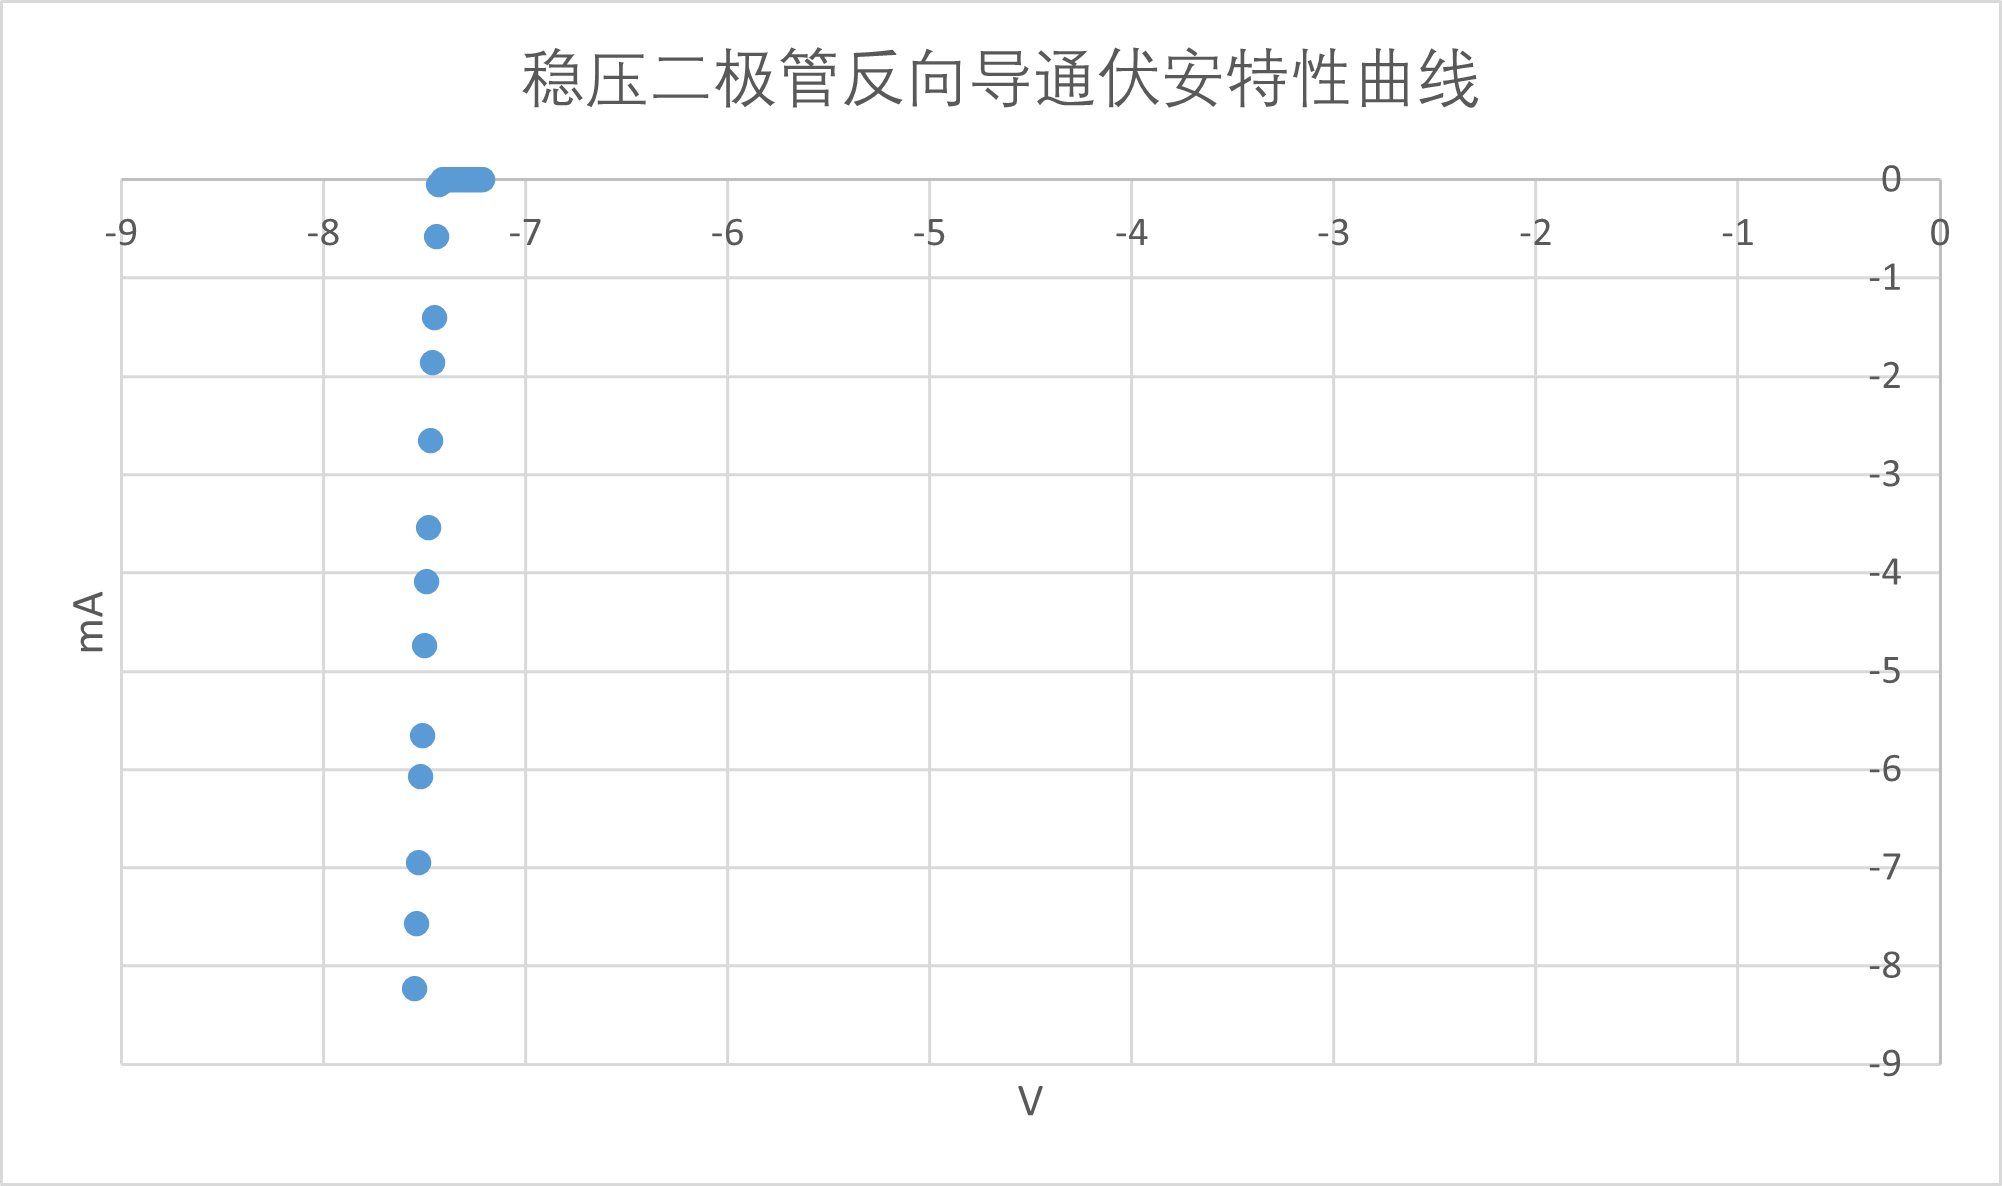
\includegraphics[width=0.4\textwidth,height=0.3\textheight]{wenyafanxiangzuotu.png}
%     \caption{稳压二极管反向导通伏安特性曲线作图}
%   \end{figure}

%   从实验结果和数据处理后形成的图像观察可以得出无论是正向导通还是反向导通,稳压二极管
%   曲线的趋势和普通二极管正向导通时候的图像是相似的,而具体而言,正向导通的导通电压阈值
%   相较于反向导通的导通电压阈值要小很多,这也体现了二极管单向导通的性质,即便是稳压二极管上
%   仍有体现。并且稳压二极管的曲线更加陡,相同电压变化下电流变化更大。
% \newpage

  \subsection{测量回路的品质因数Q值}
%   \begin{figure}[H]\label{ledshujv}
%     \centering
%     \begin{minipage}{\textwidth}
%     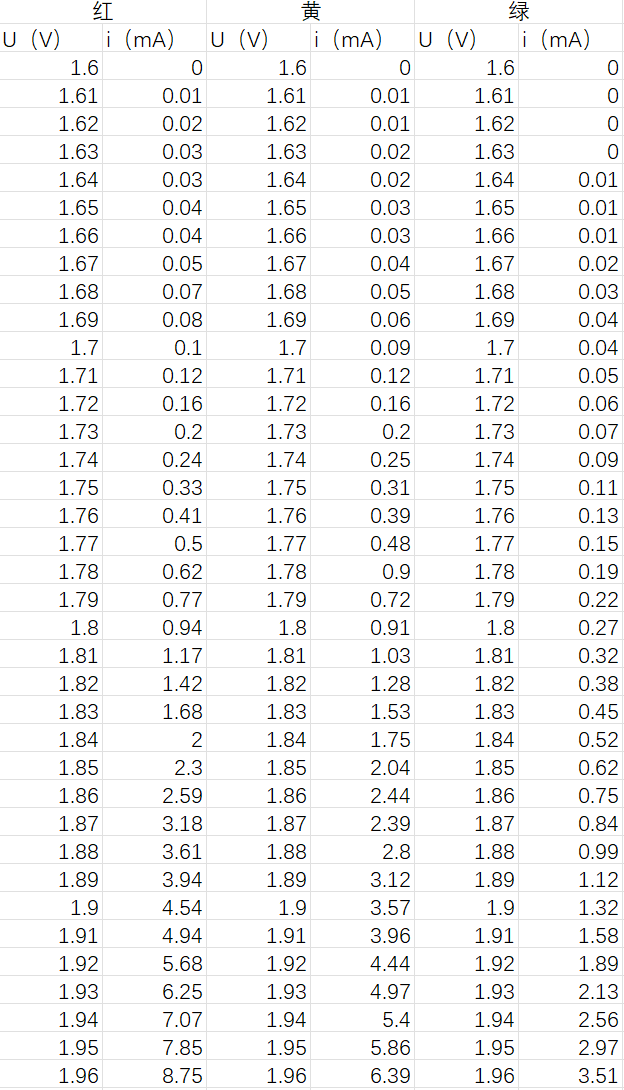
\includegraphics[width=0.2\textwidth,height=0.5\textheight]{ledshujv.png}
%     \end{minipage}
%     \caption{LED灯数据}
%   \end{figure}
%     实验中测得的LED灯的
%   伏安特性曲线数据如图\ref{ledshujv}。对数据进行处理最终得到图\ref{ledzuotu}。
%   \begin{figure}[H]\label{ledzuotu}
%     \centering
%     \begin{minipage}{\linewidth}
%     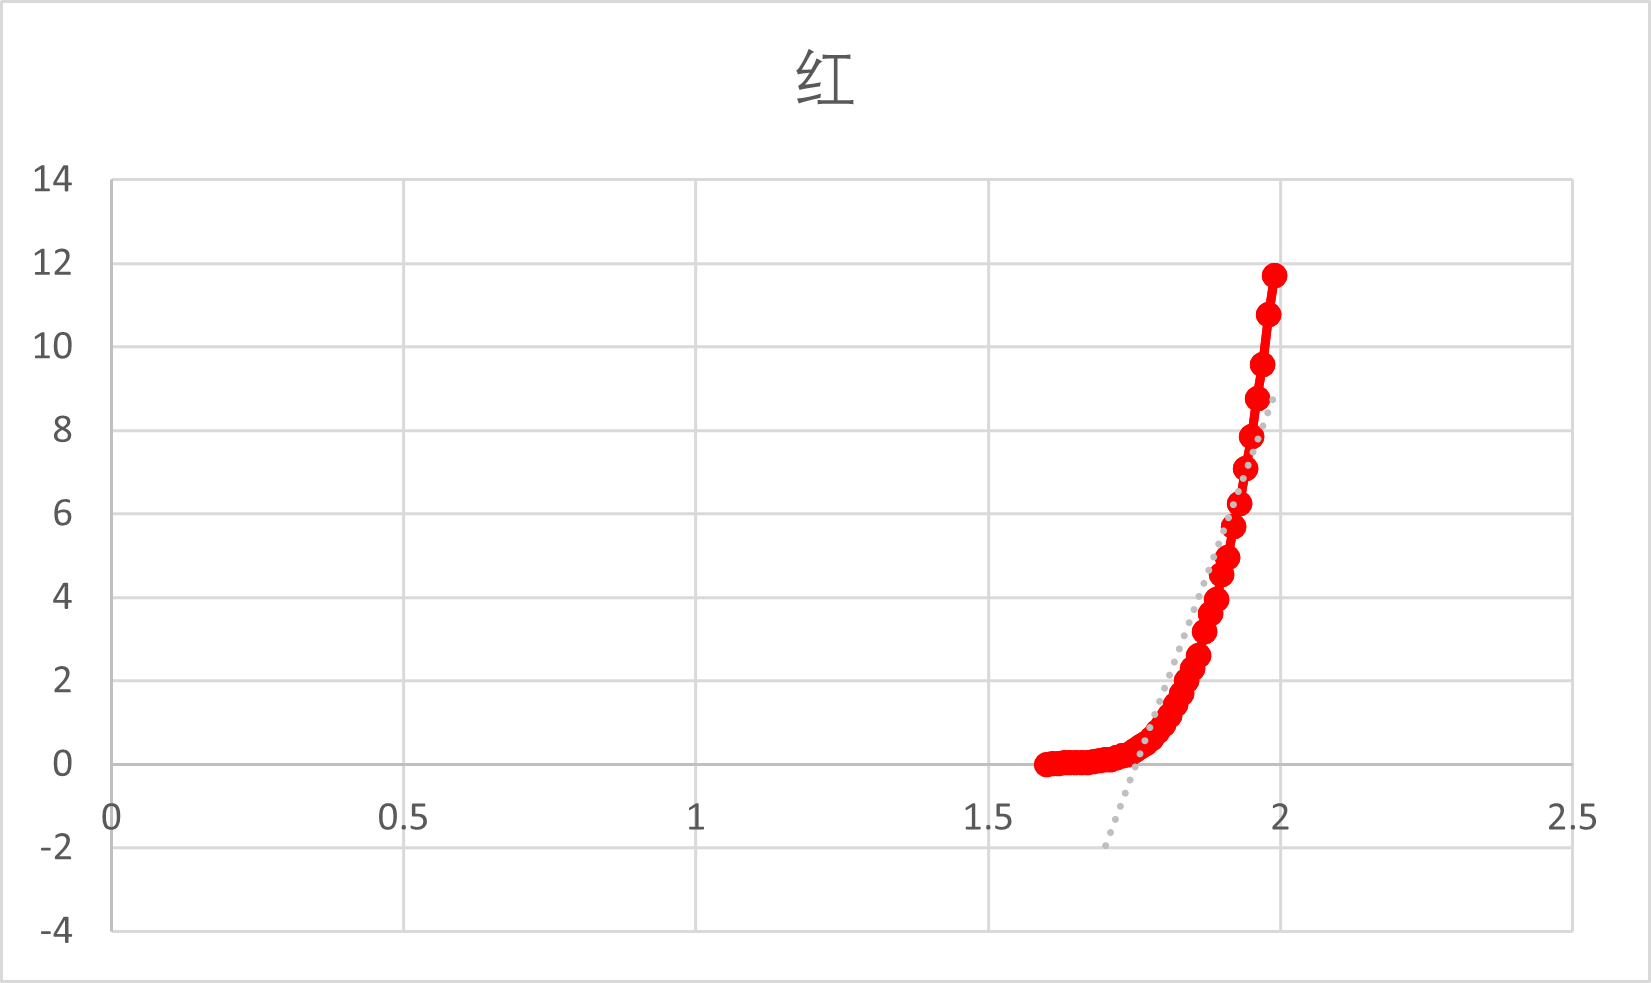
\includegraphics[width=0.47\textwidth,height=0.3\textheight]{ledzuotu1.png}\hfill
%     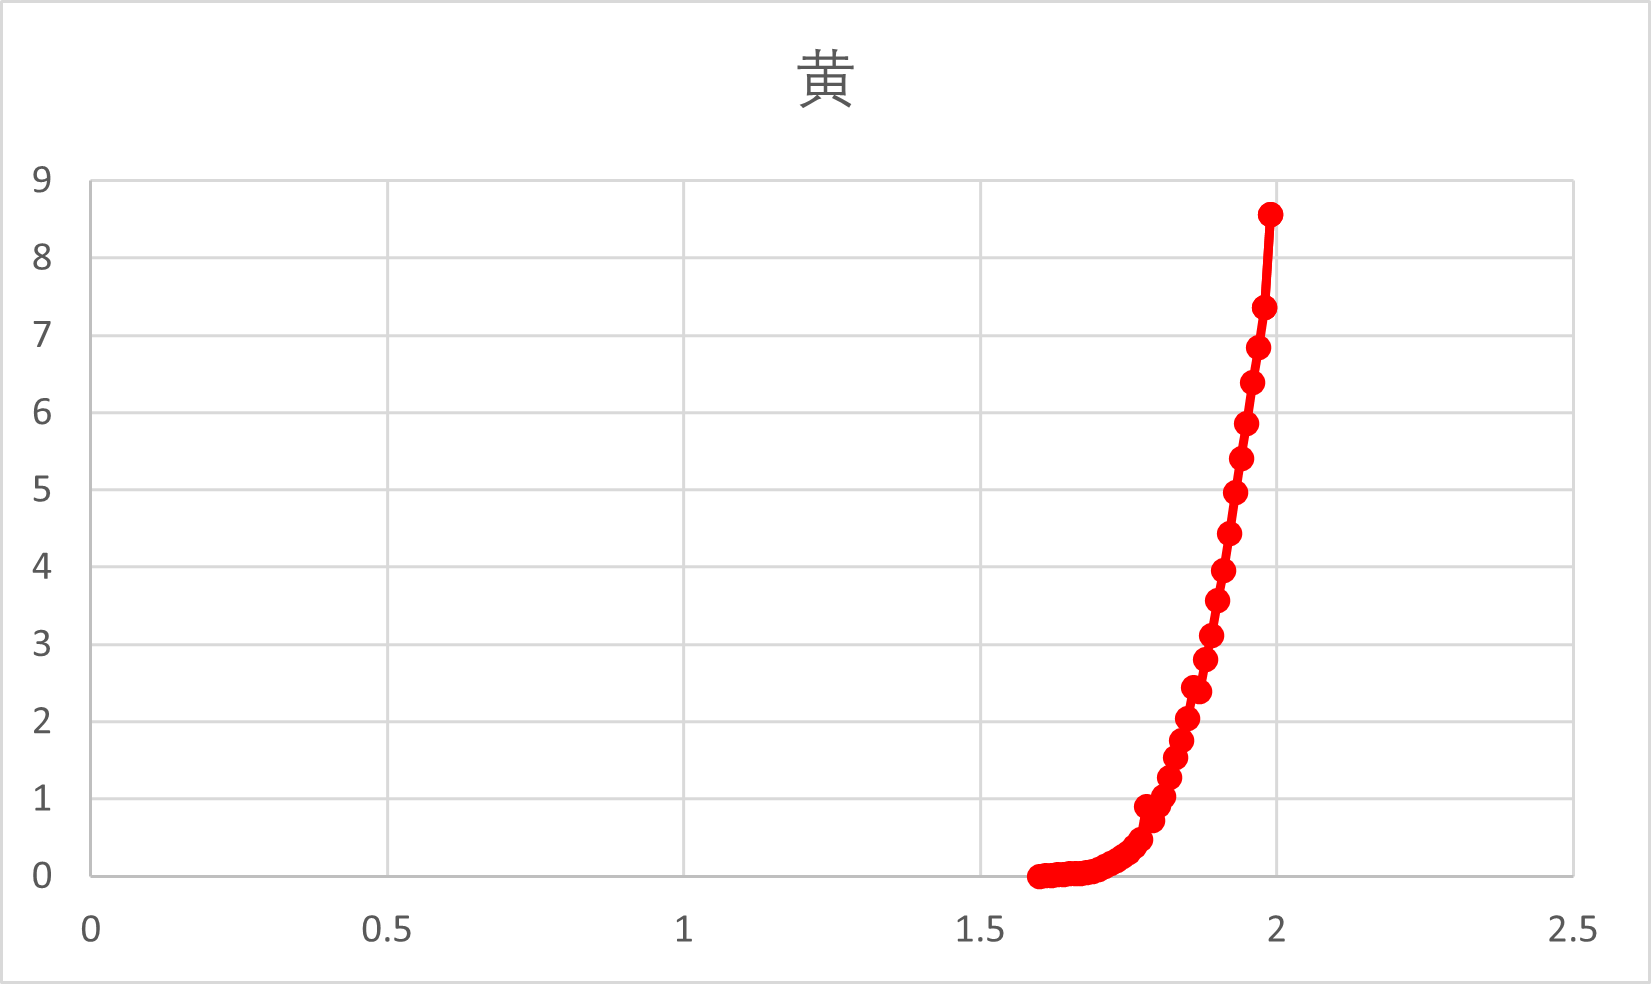
\includegraphics[width=0.47\textwidth,height=0.3\textheight]{ledzuotu2.png}\hfill
%     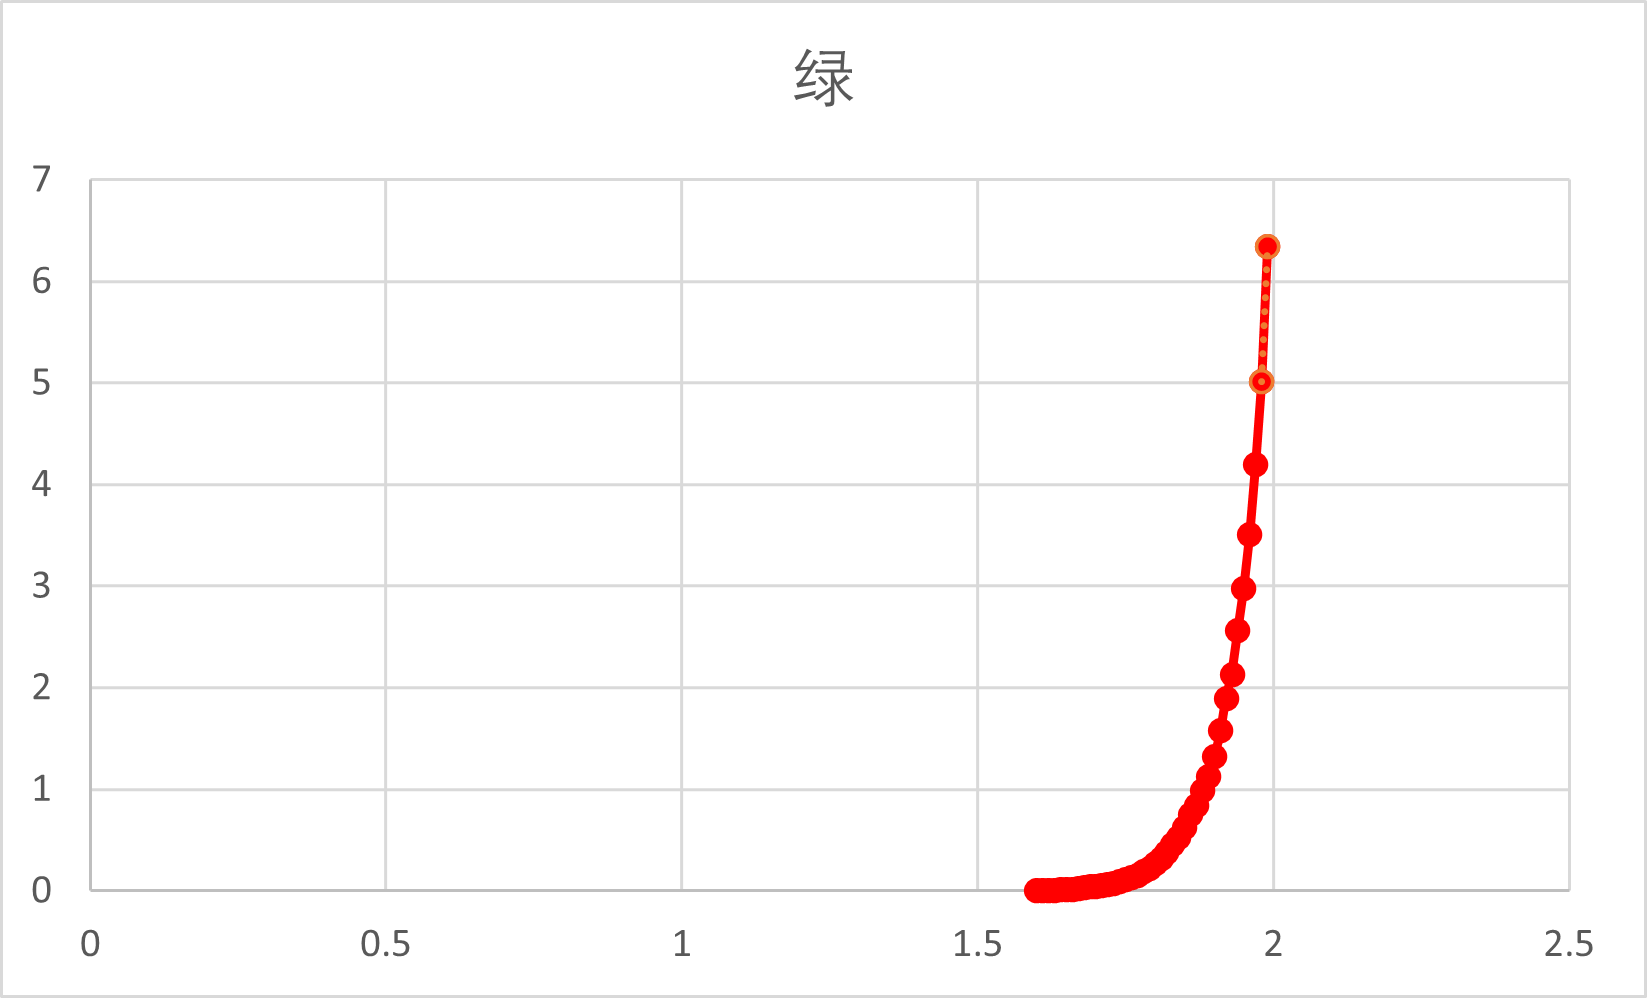
\includegraphics[width=0.47\textwidth,height=0.3\textheight]{ledzuotu3.png}
%     \end{minipage}
%     \caption{LED灯作图结果}
%   \end{figure}

%   从实验结果和数据处理后形成的图像观察可以得出无论哪种颜色的发光半导体最终产生的曲线
%   依旧和普通二极管的伏安特性曲线相似。而不同颜色的二极管的导通后的倾斜趋势不同,这也
%   体现在不同二极管的所需要的导通电压阈值不同。通过计算最终得到的灯管的波长如下表\ref{bochang}

%   \begin{table}[h]
%     \centering   
%     \caption{不同LED灯管发光波长计算}\label{bochang}
%     \begin{tabular}{| l || l |}
%         \hline
%         发光灯管颜色 & 波长数值\\
%         \hline
%         红色 & 707.567 \\
%         \hline
%         黄色 & 676.687 \\
%         \hline
%         绿色 & 644.808 \\
%         \hline
%     \end{tabular}
%   \end{table}

%   最终得到的结果误差较大,出现明显向红光偏移的趋势,分析误差产生原因:

%   1.  二极管发热导致伏安特性曲线不是相同状态下测得的

%   2.  二极管发光的时候也有红光产生,但是由于灯罩原因滤掉红光

%   3.  二极管出现故障,或者仪器误差

%   4.  测量过程中未等待二极管达到稳定工作状态就记录数据

\section{思考题}
  \subsection{思考题一}

  \subsection{思考题二}

  \subsection{思考题三}


\section{实验中个人的思考与感想}
  \subsection{对于实验个人观点}
  实验中使用的器材和书本使用不一样,所用的器材能够通过调节旋钮改变电压表所接接口。实验中可以通过在不同接口处
  连接不同电路部分而可以通过调节旋钮改变实验中电压表所接电路。虽然这样可以方便实验记录,但是实验中的电路连接会导致
  很多问题,导致实验中出现很多未知的问题。而且更多的接口也可能由于接口接触不良等问题导致实验中出现波形难以察觉的问题。

  实验中测量相位差的方式是通过调节示波器上的指针位置读取两指针之间的$\frac{1}{\Delta t}$在进行计算的方法进行实验测试。
  这其中会引入很多不确定度,在调节指针的时候也会出现很大的误差,由于很难调节两指针位置能够恰好满足实验的要求,导致实验
  误差进一步增大。当然这可能和我使用的实验器材有关,似乎隔壁几位的器材由于更为先进所以能直接读出相位差,相较于他们我实验的
  误差应该会更大。
  \subsection{实验中的总结}

\end{document}
